\pdfoutput=1
\documentclass[11pt]{article}

\usepackage{graphicx}
\usepackage[space]{grffile}
\usepackage{latexsym}
\usepackage{textcomp}
\usepackage{longtable}
\usepackage{multirow,booktabs}
\usepackage{amsfonts,amsmath,amssymb}
\usepackage{url}
\usepackage{hyperref}
\hypersetup{colorlinks=false,pdfborder={0 0 0}}
% You can conditionalize code for latexml or normal latex using this.
\newif\iflatexml\latexmlfalse
\usepackage[utf8]{inputenc}
\usepackage[english]{babel}

\usepackage{setspace}
\usepackage{apacite}
\usepackage[margin=1in]{geometry}
\usepackage{float}



\begin{document}

\title{Analysis of Dyadic Interaction in an Job Interview Setting}

\author{Suresh Alse, Bhavishya Sharma, Jay Priyadarshi, Abhishek Sharma}

\maketitle




\nocite{*}
\section{Introduction}
Interviews are often hard to be judged. It is often left in the hands of the interviewer(s) to measure the hirability of the candidates. This is fundamentally flawed as this heavily relies of interviewers' mood and personality. Also, in most cases multiple interviewers interview for the same roles which makes this process even less scientific as it is almost impossible to fairly aggregate the opinions of interviewers.

There has been tons of research by psychologists and career experts about what one should do in order to succeed in an interview \cite{huffcutt2001identification}. From this, we know that things like smiling, using a confident tone and making good eye contact can contribute a lot in an interview. However, these observations are often based on intuition and experience. Hence, It is hard to automate and quantify hirability of candidates. Also, there is a common misconception that content of the interviewee's responses is the sole determinant of the job interview. However, it is seen that non verbal aspects are as important if not more important than verbal responses \cite{mehrabian1971silent}.

\begin{figure}[h!]
\begin{center}
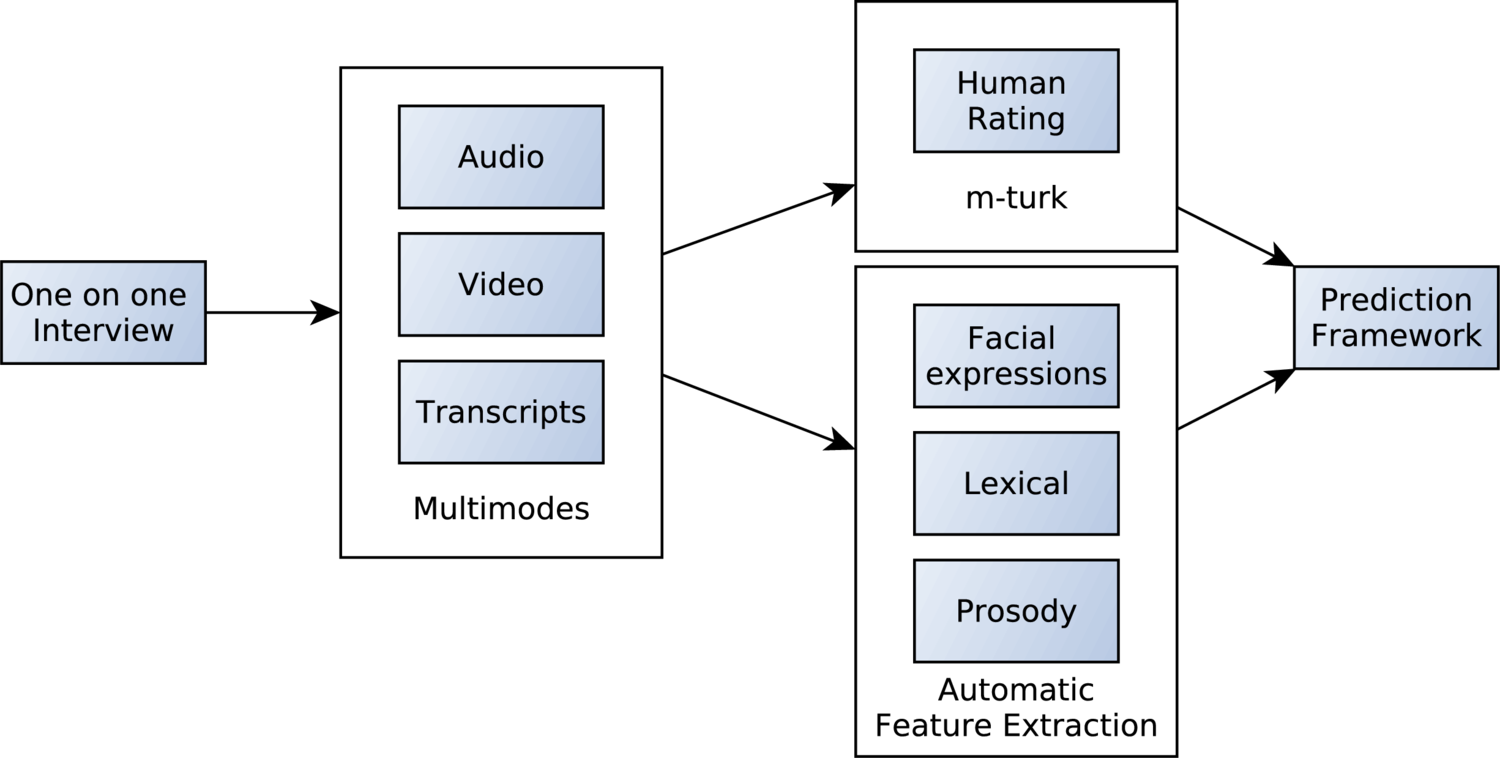
\includegraphics[width=0.7\columnwidth]{figures/process1/process1}
\label{fig:process}
\caption{{Proposed Framework%
}}
\end{center}
\end{figure}

In this project we would like to build a computational framework using which interviewers and interviewees can use it to analyze interviews and obtain the following.
\begin{itemize}
\item Automatically predict the overall score of the interview.
\item Quantify verbal and nonverbal behavior of the interviewee towards the success in the interview.
\item Automatically recommend aspects to be improved for better overall score. 
\item Timeline that shows how well the interview progressed with respect to each question.
\end{itemize}

In order to achieve this we propose a framework as shown in Figure \ref{fig:process}. We use a one on one interview data comprised of three modes (audio, video and textual). Then, we extract multimodal features (facial expressions, lexical and prosody) and predict the overall score of the interview, how likely the candidate is going to be hired and other traits required for the interview process.


\section{Related Work}
A lot of the research in the field of mulitmodal analysis of interaction has focused on speech and visual analysis of data. For instance, in Rough'n'Ready: A Meeting Recorder and Browser \cite{kubala1999rough}, they provide a way to recognize speech in the form of a BBN Byblos Speech Recognition System, where they also provide a mechanism to browse and retrieve speech data with the help of a speech index. Speaker identification is also described in The Meeting Project at ICSI \cite{morgan2001meeting}, where the acoustic model consisted of gender-dependent, bottom-up clustered (genonic) Gaussian mixtures. Further, leveraging speech recognition, topic detection in a meeting room scenario is described in Advances in Automatic Meeting Record Creation and Access, where they use a variant of Hearst's TextTiling algorithm in order to automaticaly segment the transcript into topically coherent passages.

As far as visual analysis is concerned, we can find examples of that in SMaRT: The Smart Meeting Room Task at ISL \cite{waibel2003smart}, where they provide a mechanism to track people and identify them as they move around a Meeting Room using multiple cameras and advanced computer vision techniques. Another good example of that would be Distributed Meetings: A Meeting Capture and Broadcasting System \cite{cutler2002distributed} where they augment the meeting room for remote viewers by adding cameras and other functionalities.

A major focus on such speech and visual processing (as provided above) has been focused on individuals, however, even when the researchers examine a meeting space. Our aim is to analyze dyadic communication where we don't just monitor an individual, but we attempt to find multimodal cues (such as back-channels among others) which would then uncover the underlying mechanism of a job interview.

There has been research on analyzing behavior of a group as compared to an individual, as is exemplified by research like The KidsRoom: A Perceptually-Based Interactive \cite{bobick1999kidsroom} and Immersive Story Environment and A Bayesian Computer Vision System for Modeling Human Interactions \cite{oliver2000bayesian}. However, the research here focuses on problem specific "primitive tasks", and therefore involves a much more constrained examination, which is in a sharp contrast to a sort of free-flowing, spontaneous (dyadic) interaction that we would have hoped for.

While our system focuses on some form of speech and visual processing, and also incorporates analysis of dyadic interaction as a whole, we provide a way to analyze the interaction in a much more unconstrained manner, identifying key multimodal cues, unraveling the underlying operating factors of a job interview by treating an interview as "more than a some of its parts" and hopefully, to come up with capabilities to automatically predict the overall score of an interview, quantify verbal and non verbal behavior of the interviewee towards the success in the interview, automatically recommend aspects to be improved for a better overall score, and a timeline to show how well an interview progressed with respect to time.

\section{Dataset}
We use the MIT Interview Dataset \cite{naim2015automated} for this project that we obtained by contacting the authors of the project. It consists of 138 recordings of mock interviews of students from MIT, seeking internships. The interviews were conducted in a one on one interview fashion. Both interviewers and interviewees were equipped with microphones which allows us to extract and differentiate between the speakers easily. Cameras were used to capture the video of the interviewee during the process as shown in the Figure \ref{fig:dataset}. The interviews were conducted by two professional career counselors with over five years of interviewing experience. All participants are native english speakers (this is very important because in our approach things like confidence, fluency, etc are considered). For every participant, two rounds were conducted - before and after intervention. Overall, 69 students permitted the use of recordings for research purposes. Hence we have a total of 138 recordings of lengths between 3 minutes to 8 minutes (average: 4.7 minutes per interview). Every interview consisted of interviewer asking the interviewee, five questions and no job description was given to the interviewees. The researchers who collected this data claim that this is the largest collection of job interview videos conductedby professionals.

To rate the interview, Amazon mechanical turk workers were used. Each turker watched the interview videos and rated the interviews by answering 16 assessment questions \ref{tab:assess} on seven point scale. Questions about ``Overall rating'' and ``Recommend Hiring'' captures overall score where as other questions capture higher level behavior. 
\begin{table}[h!]
    \centering
    \begin{tabular}{ | c | }
	\hline
        Engagement \\
	\hline
        Excited \\
        \hline
        Friendly \\
        \hline
        Smiled \\
        \hline
        NoFillers\\
        \hline
        RecommendedHiring \\
        \hline
        Overall \\
        \hline
        EyeContact\\
        \hline
        NotAwkward\\
        \hline
        StructuredAnswers\\
        \hline
        Calm \\
        \hline
        Focused\\
        \hline
        NotStressed\\
        \hline
        Authentic\\
        \hline
        Paused \\
        \hline
        SpeakingRate\\
        \hline
    \end{tabular} 
    \caption{Assessment questions}
    \label{tab:assess}
\end{table}

The dataset also consists of transcripts of all the interviews. This was made possible by Amazon mechanical turk workers hired by the researchers. Also, they were instructed to include filler words such as ``like'', ``uh'', ``umm'' along with cues like ``[long pause]'', ``[smiling]'' etc which are very useful for our process.

We also tried semaine-db \cite{mckeown2012semaine} which seemed good for this project. However, it just consisted data of two individuals talking to each other and was in no way an interview setting. We also considered using AMI database which consisted of a group discussing about a particular topic for a day. However, this had additional problems such as multiple people in a frame, etc and moreover similar to semaine-db, this was not a interview setting. Also, as this needs a considerable amount of data in a given setting and then requires amazon mechanical turkers, creating our own dataset seemed farfetched. Hence, we chose MIT Interview Dataset which is perfect for our project. 

\begin{figure}[h!]
\begin{center}
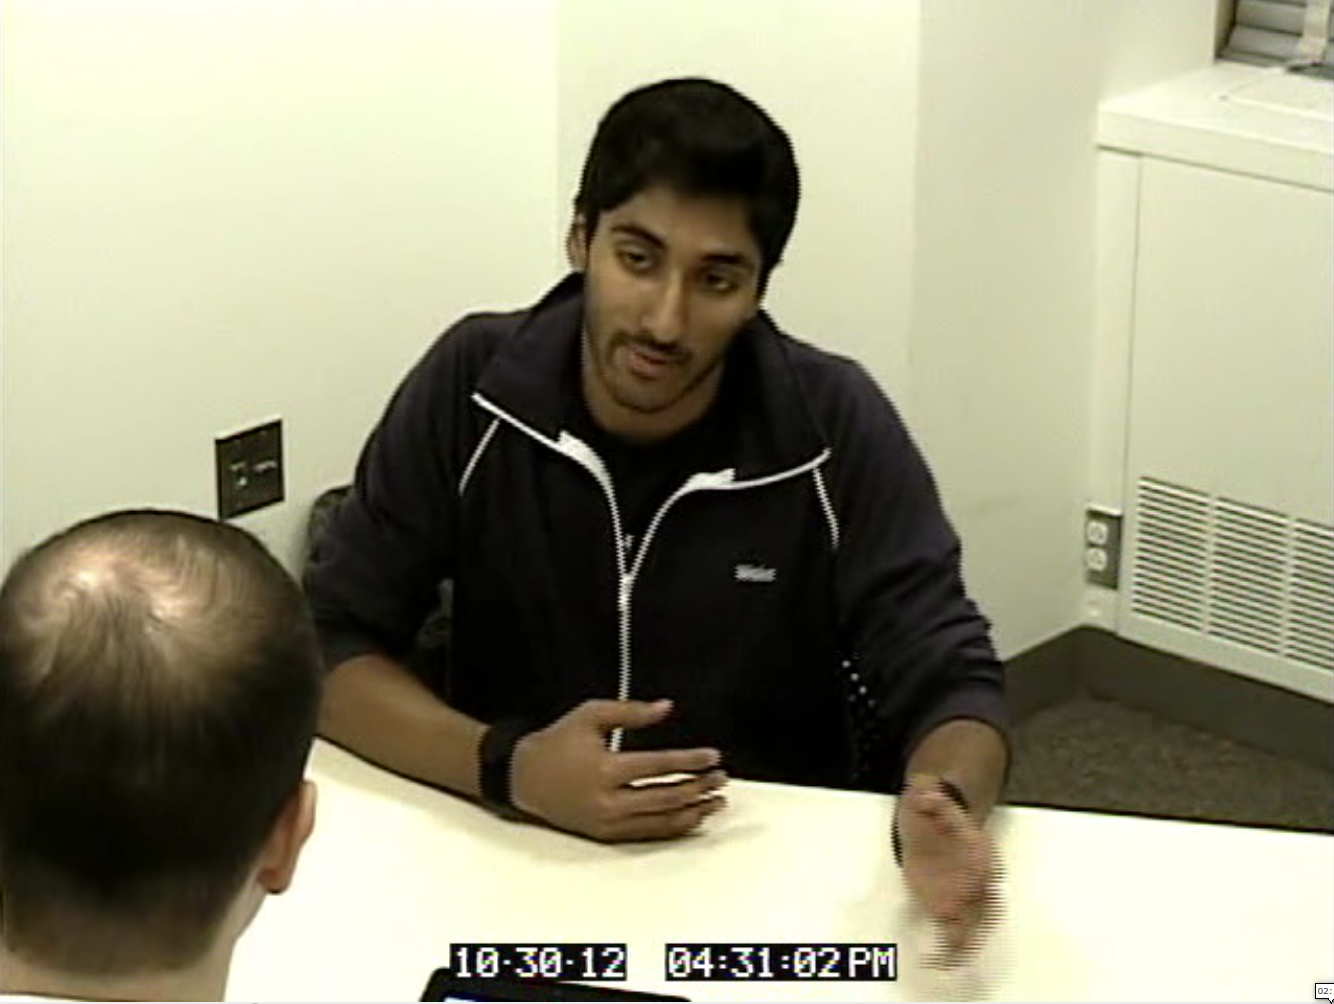
\includegraphics[width=0.5\columnwidth]{figures/Screenshot from 2016-10-21 20-30-05/Screenshot from 2016-10-21 20-30-05}
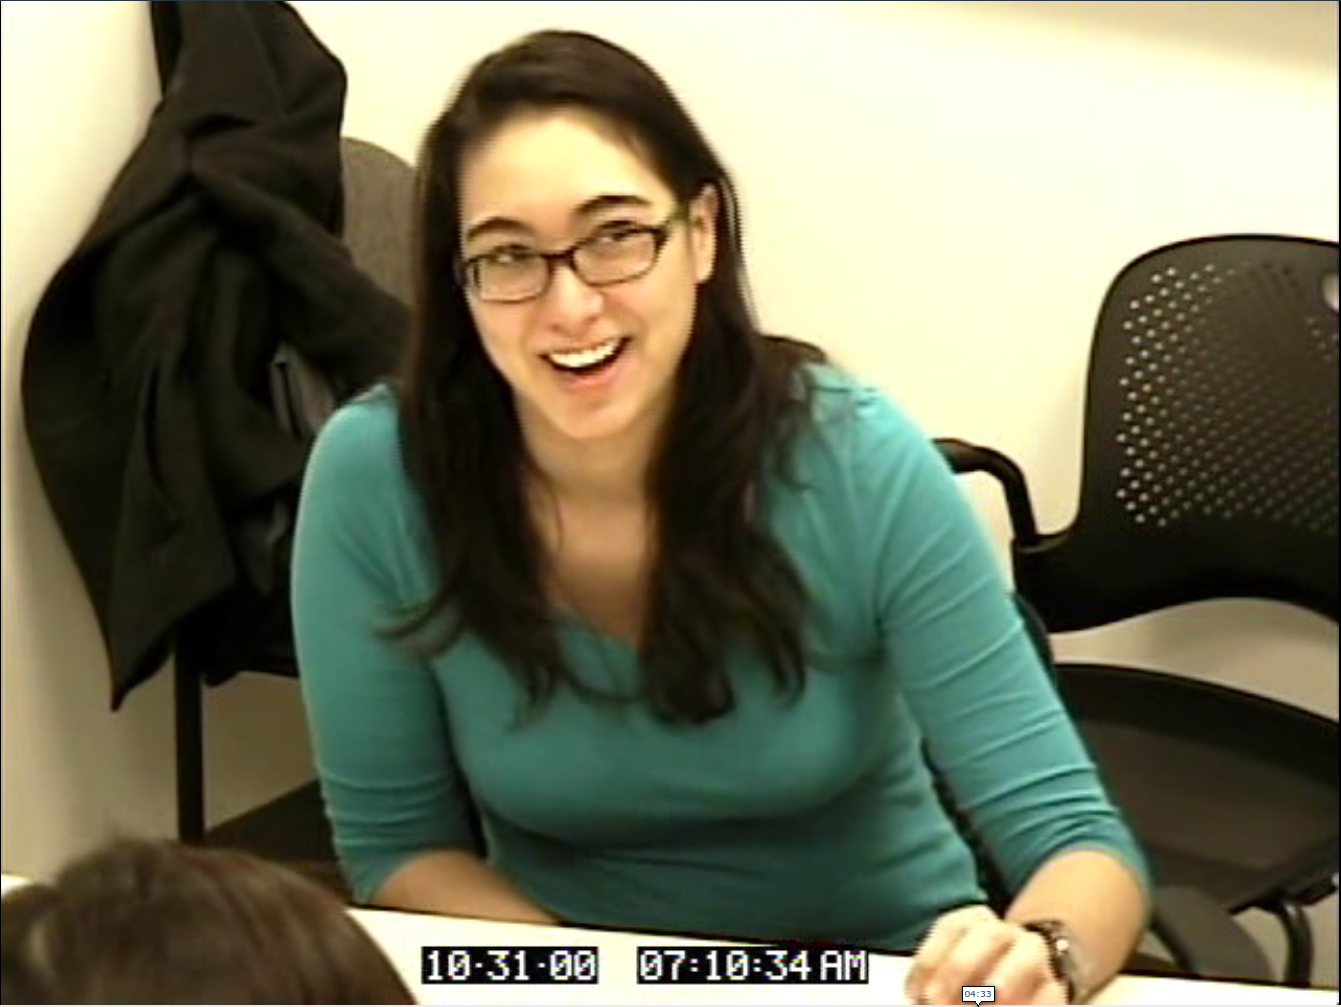
\includegraphics[width=0.5\columnwidth]{figures/Screenshot from 2016-11-28 06-21-02.png}
\caption{Two of the 138 interviews.}
\label{fig:dataset}
\end{center}
\end{figure}

\subsection{Drawbacks}
\begin{itemize}
 \item As the study is limited to undergraduate students, it might have introduced a selection bias in the dataset. 
 \item In the dataset, there are occasions where a small mistake (like using a swear word) would reflect badly on the interview outcome. As they are very rare, it is difficult to model such phenomena.
 \item The dataset has a set of 138 interviews, in which 69 interviews are before feedback is shared, while 69 are with the same participants, after the feedback is shared. This provides a bit of redundancy to an already biased dataset. As of now, we are treating each interview distinctly, however it is still up for discussion.
 \item In the dataset, the interviewer is not visible, and hence we are not able to model the interviewer’s nonverbal behavior.
\end{itemize}

\subsection{Inter-rater agreement}
To gauge the quality of the ratings given by 9 annotators, we have calculated Krippendorff’s Alpha for each trait. The ratings are on a 7-point scale. Figure \ref{fig:interrater} shows that the annotators agreed more on the if the subject had an Engaging tone, if they seemed Excited, Friendly or smiled. This can be because of the fact that we have developed necessary insticts to easily notice these things and we would almost always agree with features like if a individual smiled or if he/she was friendly or excited or even had an engaging tone. Whereas the features like Structured Answer, Authentic, Calm, paused, Speaking rate are kind of features which a lot of humans would disagree on: An idea can be Authentic to one individual might not feel Authentic to another. The same thing, measuring the Structure of an answer, Calmness, Speaking rate and Focus of an individual is something which will incur a high variance among annotators. Different annonators may have diffferent criteria for deciding the structure of an answer. Hence, it can be seen that traits like Engaging Tone, Excited, Friendly, No Fillers, Smile have good inter-annoatator agreement, where as in case of subjective traits like Structured Answer, Authentic, Stress, etc. get low scores.

\begin{figure}[h!]
\begin{center}
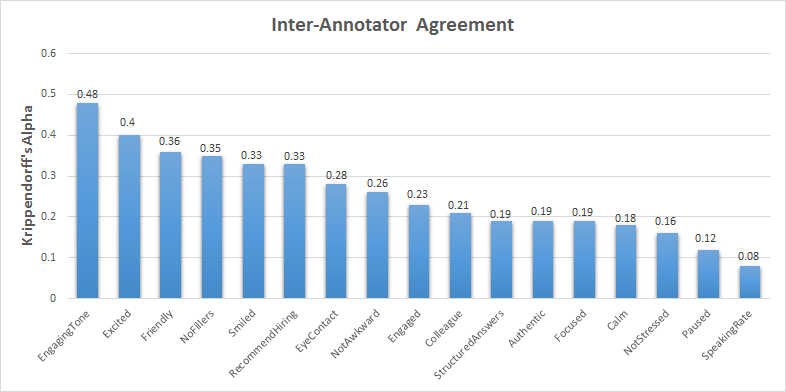
\includegraphics[width=1\columnwidth]{figures/k-alpha scores.png}
\caption{Krippendorff's Alpha}
\label{fig:interrater}
\end{center}
\end{figure}

\subsection{Feature analysis}
\label{sec:feature_analysis}
We extract Prosodic, Facial and Lexical features from the dataset as mentioned in Section \ref{sec:methodology}. Also, we did some analysis on the features extracted to get more insights to do feature selection while doing regression. For every feature we try to find the correlation between the features and the scores of assessment questions.
\subsubsection{Prosodic Features}
The extracted prosodic features consists of energy, power, pitch etc. Every interview is divided into five segments corresponding to five different questions asked by the interviewer. After averaging out all the features for each of the segments, we try to match it with the scores assigned by the turkers for each of the assessment questions. We draw a scatter plot and try to fit a line to see how relevant the score is to each of these features. A positive slope indicates that with the increase in the value of the feature, a higher score would be assigned. A negative slope would indicate that with the increase in the value of the feature, a lower score would be assigned. A near zero slope would indicate that this feature wouldn't matter and we can neglect it in regression. Figures \ref{fig:prosodic_analysis1}, \ref{fig:prosodic_analysis2}, \ref{fig:prosodic_analysis3} and \ref{fig:prosodic_analysis4} are some of the 1026 graphs that were drawn to visualize this. In Figure \ref{fig:prosodic_analysis1} we can see that with the increase in energy, interviewees are likely to be more excited. Figure \ref{fig:prosodic_analysis2} indicates that the recommended rating score drops with the increase in shimmer. Figure \ref{fig:prosodic_analysis4} indicates that Min pitch and Engaged score are not related and hence we can ignore it. 

\begin{figure}[H]
\begin{center}
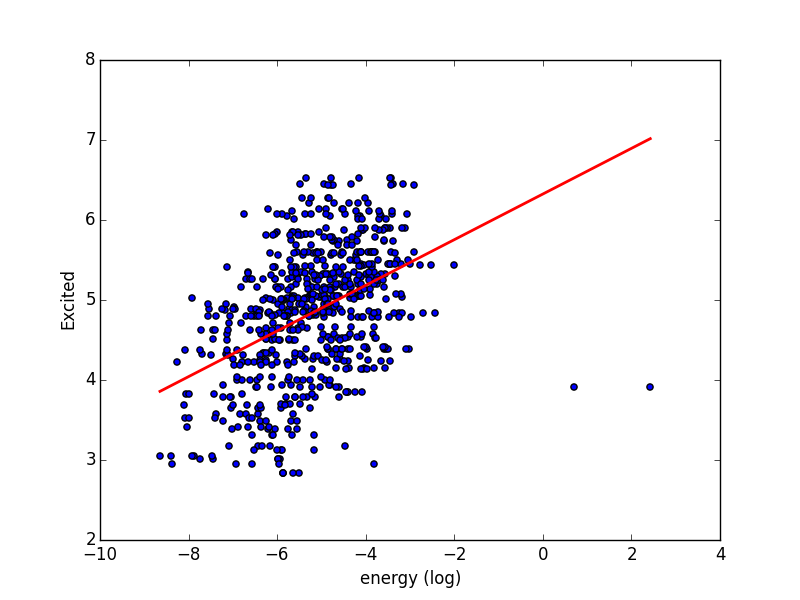
\includegraphics[width=0.5\columnwidth]{figures/Excited and energy.png}
\caption{Energy vs Excited}
\label{fig:prosodic_analysis1}
\end{center}
\end{figure}

\begin{figure}[H]
\begin{center}
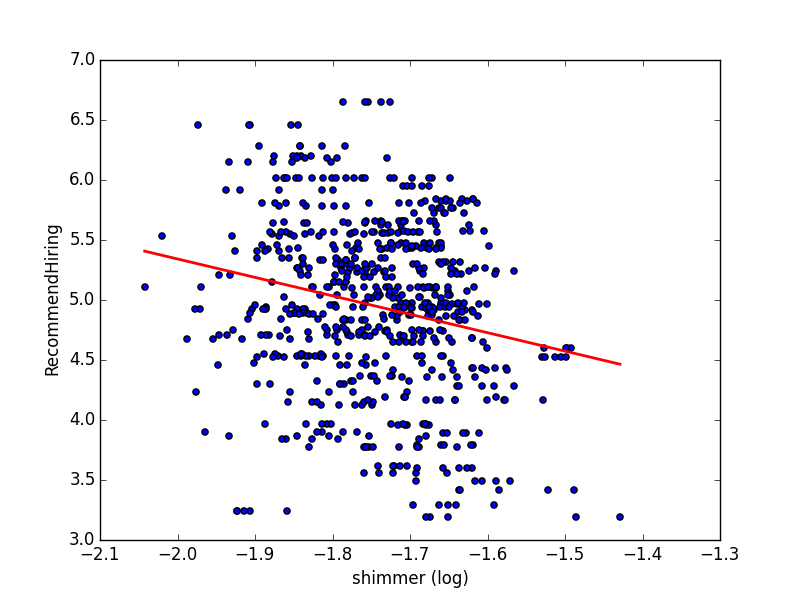
\includegraphics[width=0.5\columnwidth]{figures/RecommendHiring and shimmer.png}
\caption{Shimmer vs Recommended Hiring}
\label{fig:prosodic_analysis2}
\end{center}
\end{figure}

\begin{figure}[H]
\begin{center}
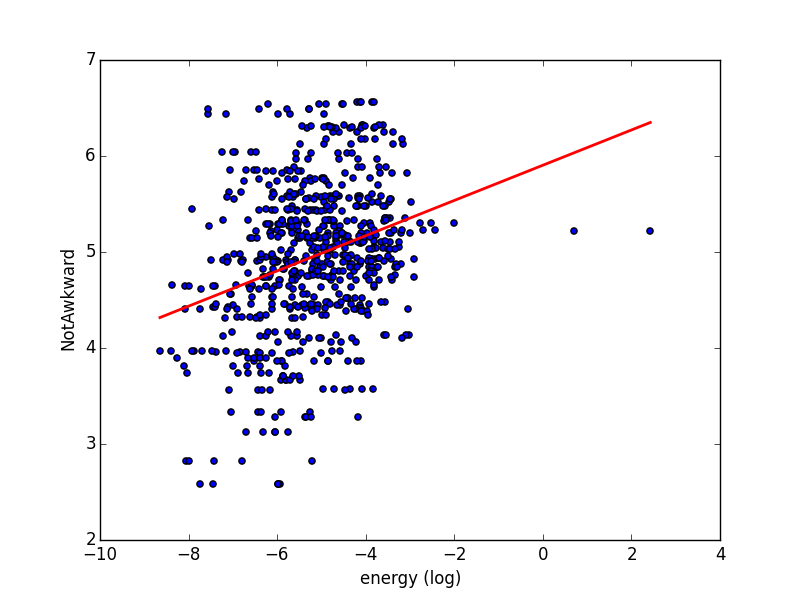
\includegraphics[width=0.6\columnwidth]{figures/NotAwkward and energy.png}
\caption{Energy vs NotAwkward}
\label{fig:prosodic_analysis3}
\end{center}
\end{figure}

\begin{figure}[H]
\begin{center}
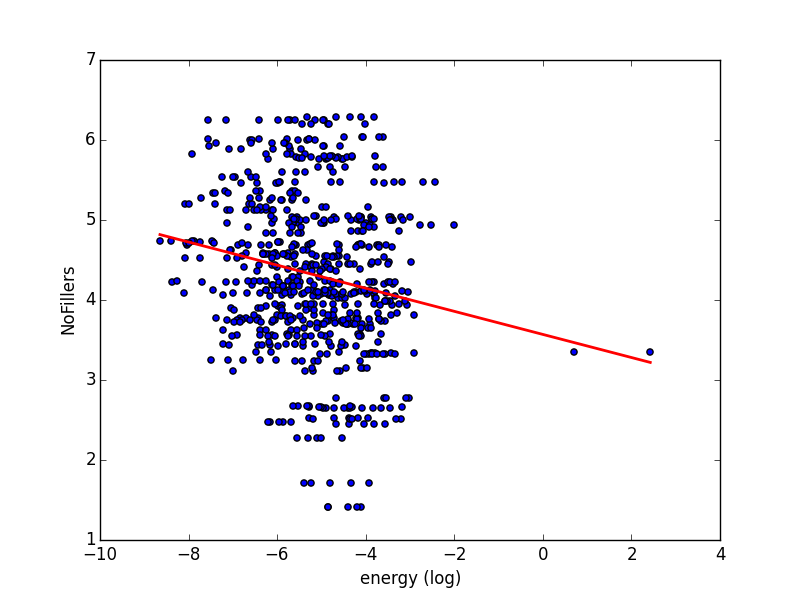
\includegraphics[width=0.6\columnwidth]{figures/NoFillers and energy.png}
\caption{Energy vs No. of Fillers}
\label{fig:prosodic_analysis5}
\end{center}
\end{figure}


\begin{figure}[H]
\begin{center}
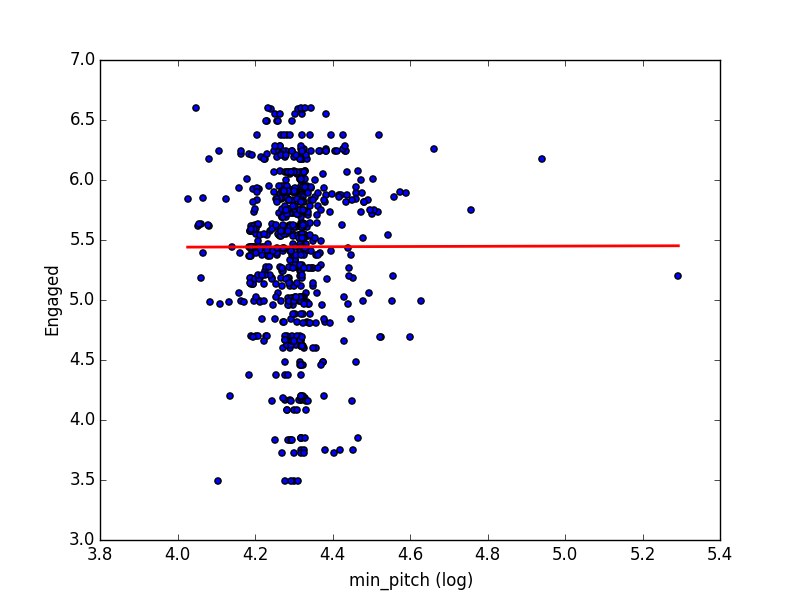
\includegraphics[width=0.6\columnwidth]{figures/Engaged and min_pitch.png}
\caption{Min Pitch vs Engaged}
\label{fig:prosodic_analysis4}
\end{center}
\end{figure}

As we observe direct correlation between these extracted features, we can consider these directly in our approach.

\subsubsection{Facial Features}
Facial features extracted are composed of features such as pitch, yaw, roll etc of the face at every frame. By taking average of the features of the frames corresponding to every question we do similar analysis as we did in case of prosodic features. Figure \ref{fig:facial_analysis} shows how pitch of the face varies with engaged.

\begin{figure}[H]
\begin{center}
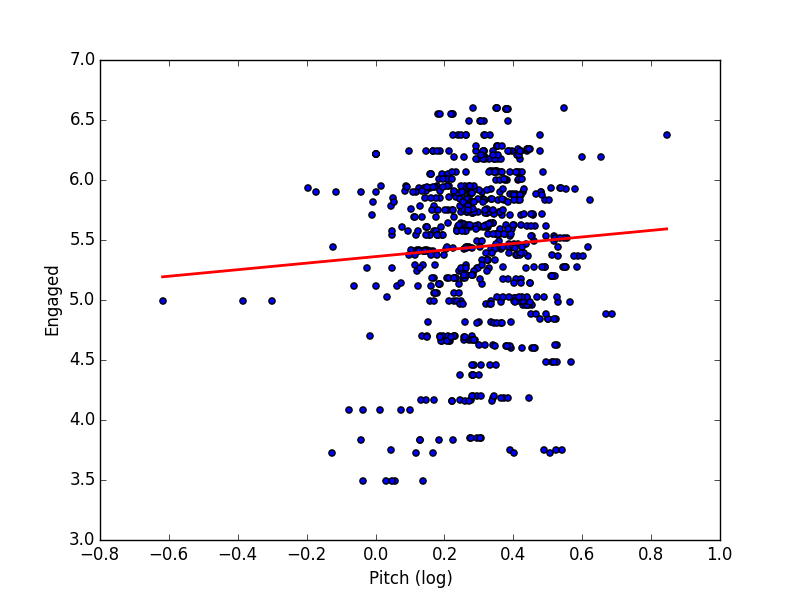
\includegraphics[width=0.6\columnwidth]{figures/Engaged and Pitch.png}
\caption{Pitch vs Engaged}
\label{fig:facial_analysis}
\end{center}
\end{figure}

We see that this approach doesn't give much insights about the assessment questions. So, we can't just use these features and we have to do some feature extraction from these features which we describe in Section \ref{sec:methodology}.
\subsubsection{Using Logistic Regression}
Although visual analysis gives us some insights which will help us for feature selection, it is not very scientific and it does not work well with visual features. We also tried using statistical measures such as t-test, kstest and kl divergence which didn't give any significant improvement over visual analysis. Hence we used logistic regression. 

We create a feature vector of all the features including prosodic, lexical and facial features and train a logistic regression classifier for each of the assessment questions as shown in the Figure \ref{fig:logistic_regression}. We use the score assigned by turkers rounded off to nearest whole number as the class of the feature vectors. For every assessment question we have a separate logistic regression classifier. After the models are trained, the coeffecients of the features indicate how important a given feature is to score the assessment question. Note that a negative score indicates that the feature impacts the assessment question negatively and doesn't mean that it is less important. Hence we take the absolute values of the coeffecients as the measure of importance.

\begin{figure}[H]
\begin{center}
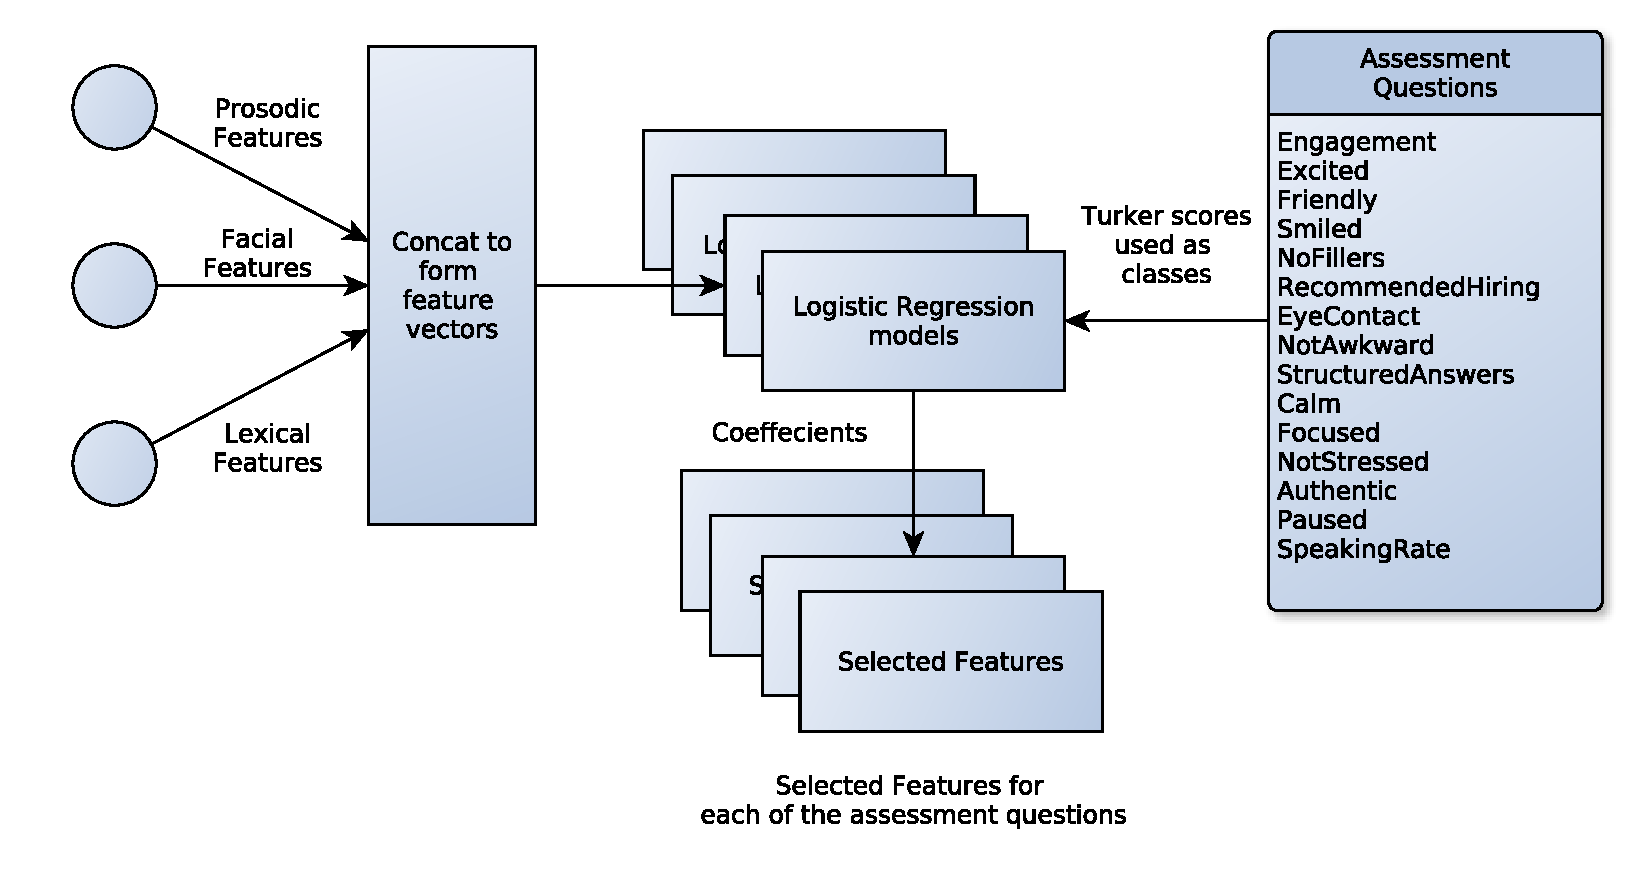
\includegraphics[width=0.8\columnwidth]{figures/logistic_regression.pdf}
\caption{Using Logistic Regression to select features for each of the assessment questions}
\label{fig:logistic_regression}
\end{center}
\end{figure}
From the combination of visual analysis and the coeffecients we select the best set of features for SVR manually. For instance ``head\_nod'', ``head\_shake'', ``mean\_pitch'', ``pitch\_sd'', ``Yaw'' and ``Roll'' are considered as features for ``Engaged'', ``energy'', ``power'',``intensityMean'', ``intensitySD'', ``mean\_pitch'' and ``pitch\_sd'' are consided as features for ``Excited'' and so on.

\section{Methodology}
\label{sec:methodology}
This section we describe the overall approach towards building the proposed framework.

\subsection{Feature Extraction}
We consider three categories of features in our approach i.e Prosodic features, lexical features and facial features. Also, as the data provides with necessary transcripts from m-turkers along with filler words, we don't have to use any automatic speech recognition. Hence lexical features can be extracted directly from transcripts.
\subsubsection{Prosodic Features}
In order to extract prosodic features from the audio, we used an open source speech analysis tool called PRAAT \cite{naim2015automated}. From the dataset we know the durations of each of the question asked during the interview. So each interview can be divided into five parts. We extract prosodic features over these five parts and keep it separately.

According to some of the previous research \cite{frick1985communicating}, pitch, intensity, characters of first three formants and spectral energy are found to be more representative of our behavior. For every feature we extracted mean, variance, minimum and maximum values. We also extracted additional features such as pauses, non-uniform pitch and intensity of speeches as it will help in determining overall score of the interview.
\subsubsection{Lexical Features}
Word count is often used as lexical feature in many applications. However, we only have limited data; hence, we will not be able to use it as it would result in sparse high dimentional feature vectors. To resolve this problem, we will use Latent Dirichlet Allocation (LDA) to learn 20 topics from interview dataset. Then, we use the relative weights of these topics in every interview as lexical features.

Also, we know that speaking rate and fluency can be indicators of a good interview. Hence, also use additional features such as words per second, unique words per second, filler word count and unique word count. 
\subsubsection{Facial Features}
Facial features are very important and are hard to be quantified. In this project, we extract features from every frame in the video sequence. The dataset includes the facial features extracted for each video using Shore framework. We will divide every video into five parts corresponding to the questions asked. The dataset also consisted of smile data of faces represented by a value between 0-100. Additionally, We extracted head gestures such as nods and shakes from each video frame, and treated their average values as features.

We will normalize all the features to have zero mean and unit variance to eliminate bias.

\subsection{Score Predictions}
We use the features extracted as mentioned above to predict the final score.
\subsubsection{Training}
Figure \ref{fig:methodology-training} shows the overall approach for training. We treat aggregate of every assessment question scored by the turkers as a feature and concatenate them to form a feature vector. The overall score rounded to nearest score in the 1-7 point scale is considered as the training class. We use the feature vector and the the score to train a SVM model which can be used to predict scores.
\begin{figure}[h!]
\begin{center}
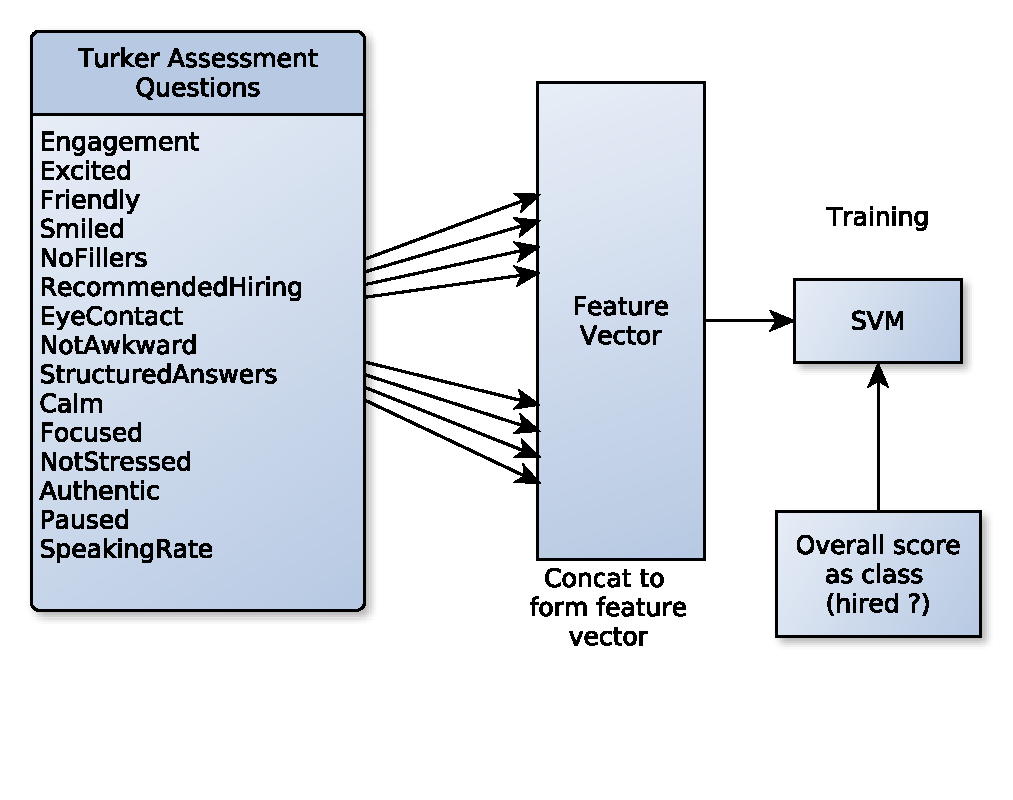
\includegraphics[width=0.7\columnwidth]{figures/methodology-training.pdf}
\caption{Training}
\label{fig:methodology-training}
\end{center}
\end{figure}
\subsubsection{Classification}
After training the SVM model we will use it as mentioned in the Figure \ref{fig:methodology} for prediction. After extracting the multimodal features, we will perform feature selection as mentioned in Section \ref{sec:feature_analysis} to select appropriate features for each of the assessment questions. We will use SVR type of regression to predict the scores for assessment questions. Assessment scores used to train the SVM model is used to train SVR as well. While predicting the scores of assessment questions, we do it on question level i.e every question asked by the interviewer. Once, we have the assessment question scores, we concatenate it to form a feature vector. This is then passed to SVM classifier trained earlier to predict the final score. For every interviewee, we will have five results corresponding to each question. The average score is considered to see if the interviewee should be hired or not.

\begin{figure}[h!]
\begin{center}
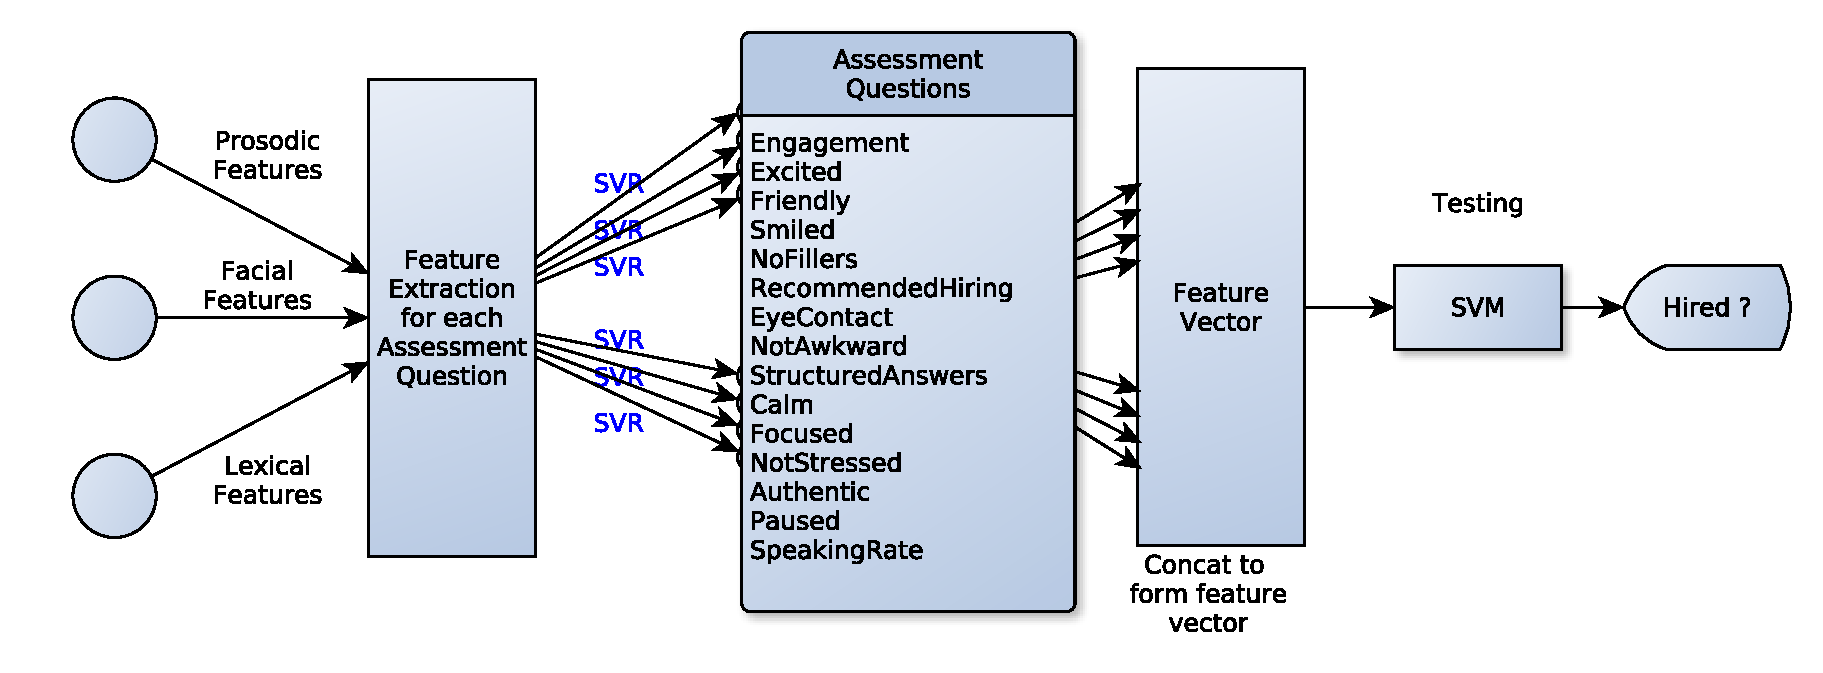
\includegraphics[width=1\columnwidth]{figures/methodology.pdf}
\caption{Prediction}
\label{fig:methodology}
\end{center}
\end{figure}

\subsubsection{Score analysis}
Now that we have predicted scores from both regression and classification we can get granular insights for job interviews. From SVM, we can get the overall hiring rating. We can recommend a person for hiring if the overall rating is greater than or equal to 5/7. From regression we get how well the interviewee has done in each of the assessment questions categories. So we can know the strength and weaknesses of the candidate in each of these categories. From logistic regression we know the ranking of features for regression. Using this we can give very specific details in each of these categories where the interviewee has or hasn’t done well or can improve. 

\subsubsection{Validation}
We divide the data into training and test sets. 75\% of random samples from the data is used for training and the remaining 25\% is used for testing. We use 3-fold cross validation in both SVR and SVM models as shown in the Figure \ref{fig:validation} to estimate the hyper-parameters. In SVR we do cross-validation to estimate $\gamma$, $C$ and $\epsilon$ and in case of SVM we do cross-validation to estimate $C$.
\begin{figure}[H]
\begin{center}
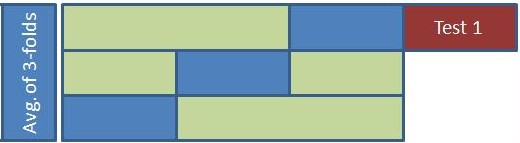
\includegraphics[width=0.6\columnwidth]{figures/validation.jpeg}
\caption{3-fold Cross Validation with test set}
\label{fig:validation}
\end{center}
\end{figure}
\subsection{Results}
In this section we will show the results of our approach across different steps.
\subsubsection{Support Vector Regression}
We use SVR to predict the values of assessment questions as mentioned in the previous sections. To analyse the result we draw three graphs for every assessment question. This is mainly done because we do not have any other work which we can compare these results with and have to rely on our analysis to make sure that we have accurate results to move forward in the process. Every graph has interview \# on the x-axis representing every interview. The first graph represents the difference between the predicted score and the actual score (aggregate turker score) for a given assessment question. 
\begin{equation}
 f_1(i) = predicted(i) - turker(i)
\end{equation}
Although the first question gives us some idea about how close the predicted values are to the turker assigned scores, we draw another graph to take a closer look. In this graph we round the scores before taking the difference. This helps us visualize the difference after weeding out the close matches.
\begin{equation}
 f_2(i) = round(predicted(i)) - round(turker(i))
\end{equation}
We also find the accuracy based on these rounded values.
\begin{equation}
 accuracy = \frac{count(round(predicted(i)) == round(turker(i)))}{\textit{number of interviews}}
\end{equation}
To take an even closer look we draw another graph. As mentioned before every score is between 1-7 scale. We would like to see how close the predictions would be if we consider the given assessment question alone for hiring. We consider an interviewee hired if they score (in the assessment question and not the overall score) a value greater than or equal to 3. Note that this is only to analyse the output of the regression and will not be used in any way in further steps.
\begin{equation}
     f_3(i) = \left\{
                \begin{array}{ll}
                  1 \textit{ if predicted(i)} \geq 3 \textit{ and  turker(i)} \geq 3\\
                  1 \textit{ if predicted(i)} < 3 \textit{ and  turker(i)} < 3\\
                  0 \textit{ otherwise}\\
                \end{array}
              \right.
\end{equation}
We also find accuracy of predicting this. We call it \textit{Hired Accuracy}.
\begin{equation}
 accuracy_{hired} = \frac{count(f_3(i) == 1)}{\textit{number of interviews}}
\end{equation}
The following figures contain graphs mentioned above along with accuracy and hired accuracy for every assessment question.



\begin{figure}[H]
\begin{center}
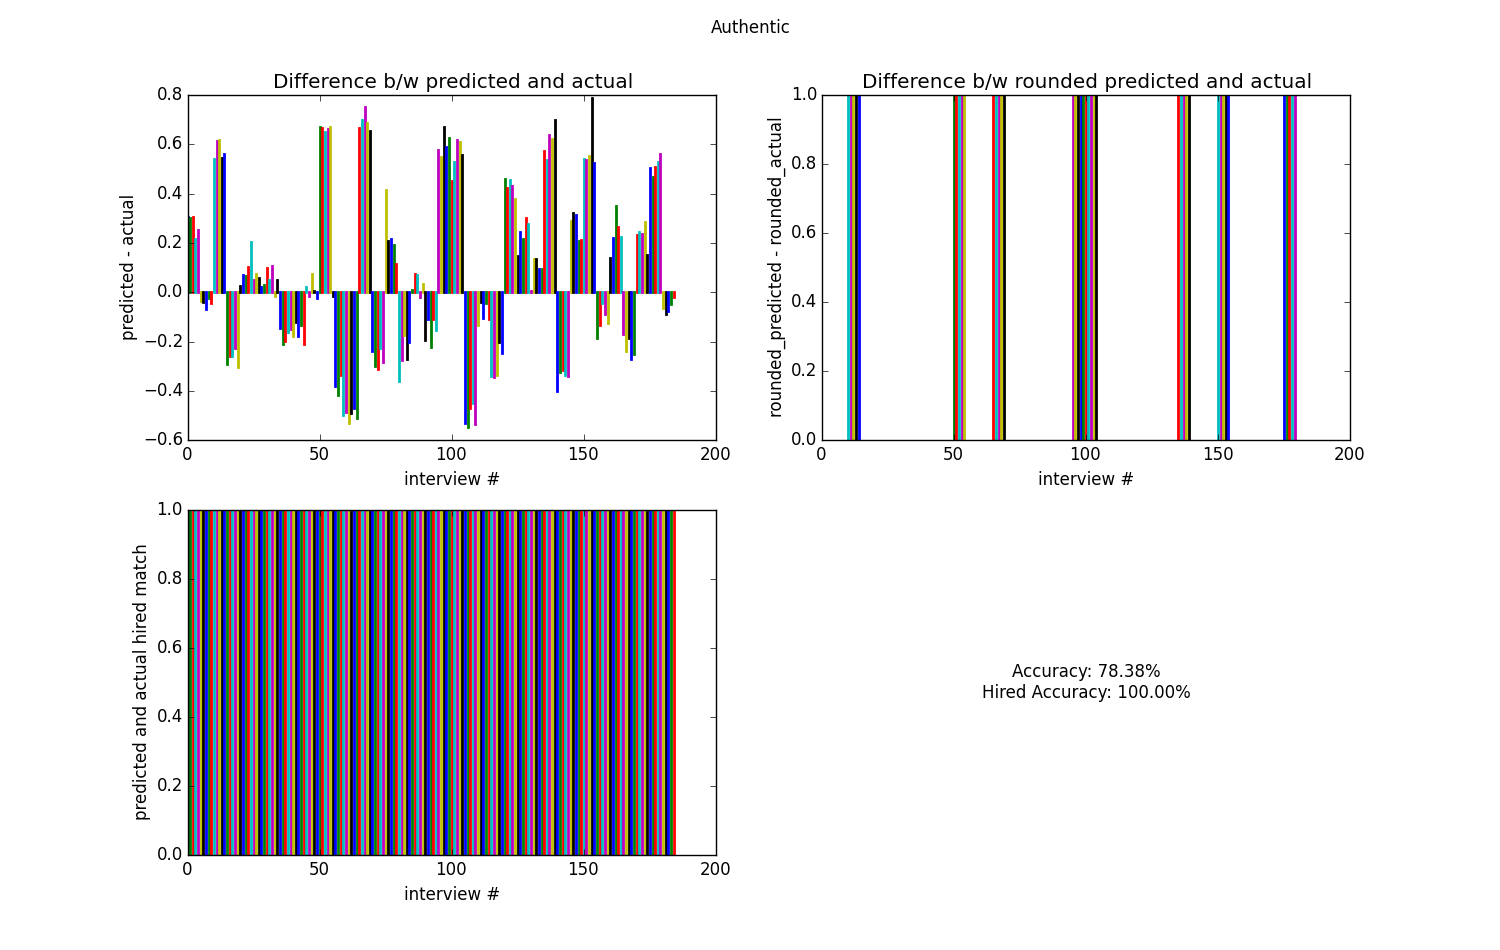
\includegraphics[width=1\columnwidth]{figures2/Authentic.png}
\caption{This shows the results for the assessment question - Authentic. From the first graph we see that there is a difference between predicted and actual scores as expected. While comparing the rounded values, we see that there are a lot of interviews with value 0 i.e we were able to successfully predict scores for those case. Accuracy for this case was found to be 78.38\%. From the third graph we can see that we get a hired accuracy of 100\% as all the values in the graph are equal to 1}
\label{fig:Authentic_svr}
\end{center}
\end{figure}

Similar to Figure \ref{fig:Authentic_svr}, we draw graphs along with accuracy and hired accuracy to visually analyse the predicted scores from support vector regression for every assessment question.

\begin{figure}[H]
\begin{center}
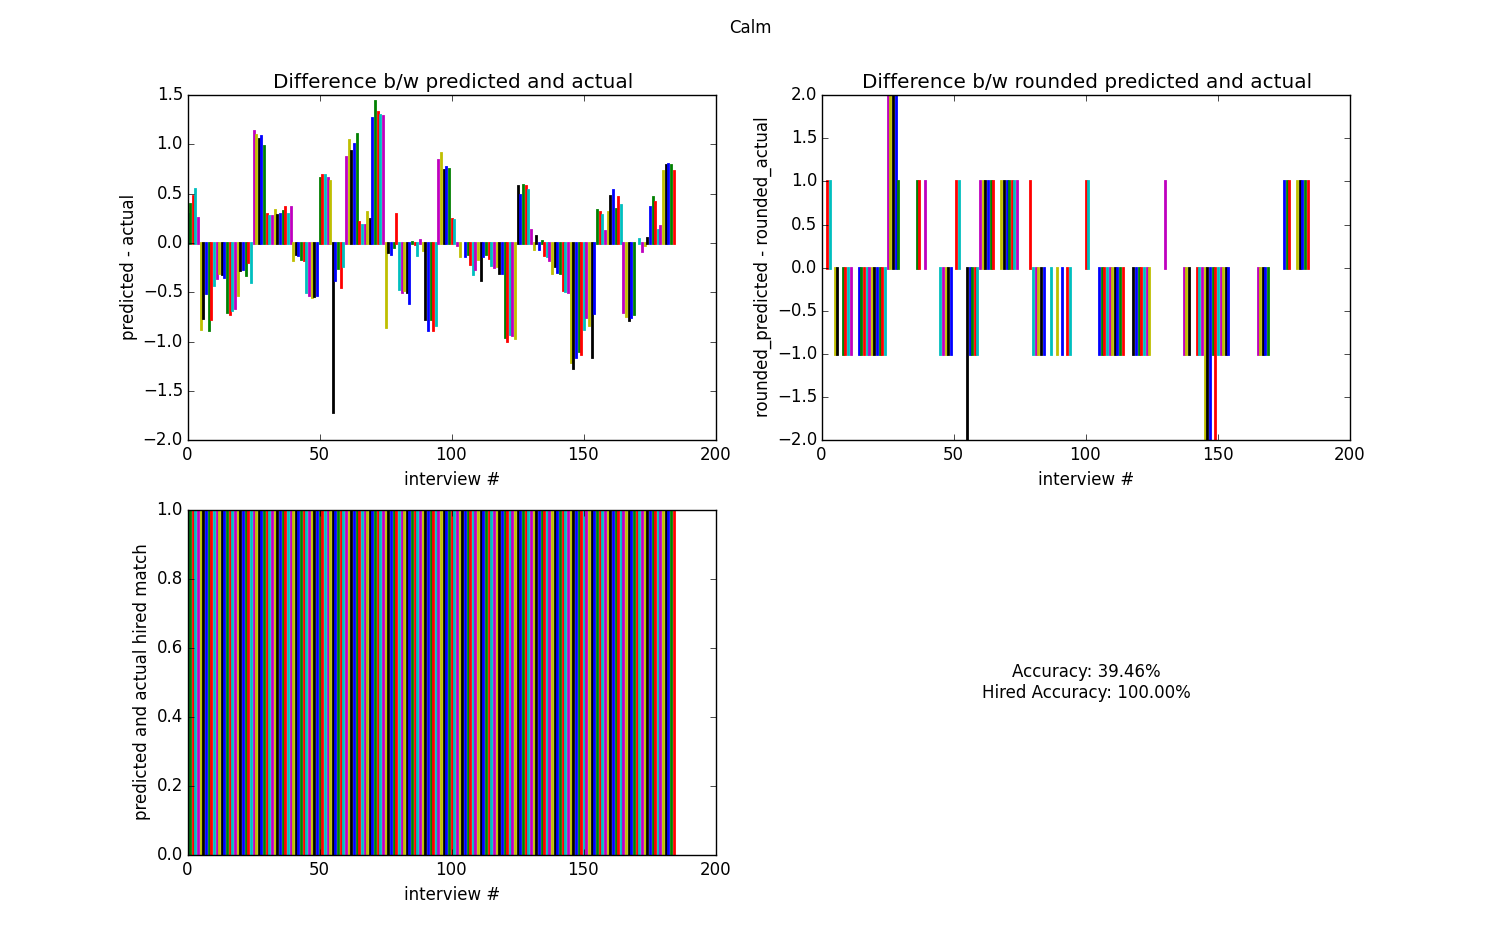
\includegraphics[width=1\columnwidth]{figures2/Calm.png}
\end{center}
\end{figure}

\begin{figure}[H]
\begin{center}
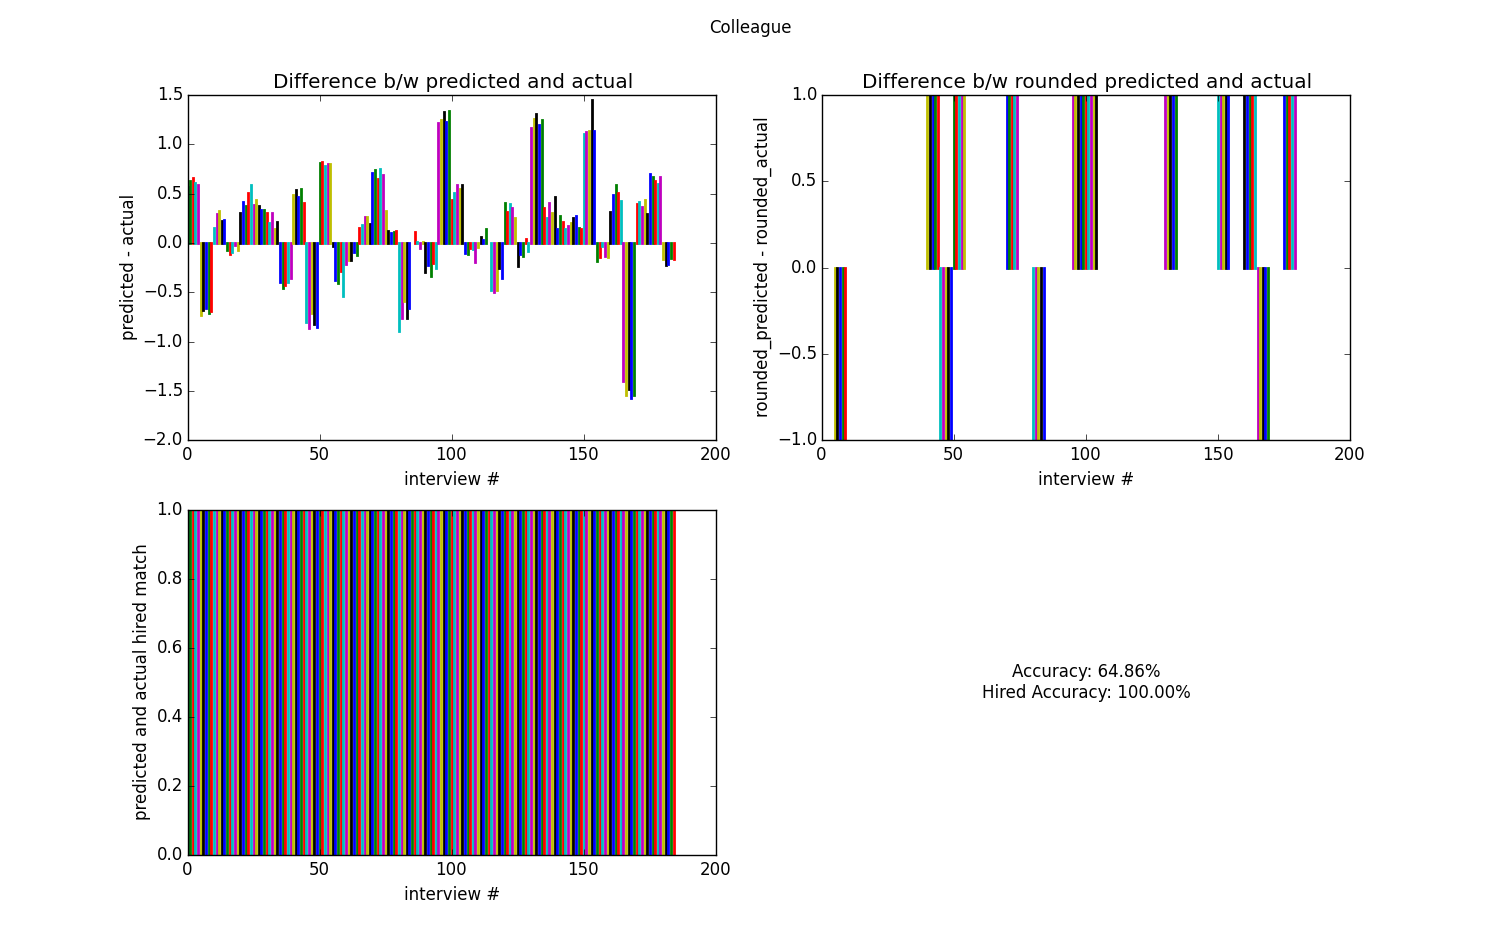
\includegraphics[width=1\columnwidth]{figures2/Colleague.png}
\end{center}
\end{figure}

\begin{figure}[H]
\begin{center}
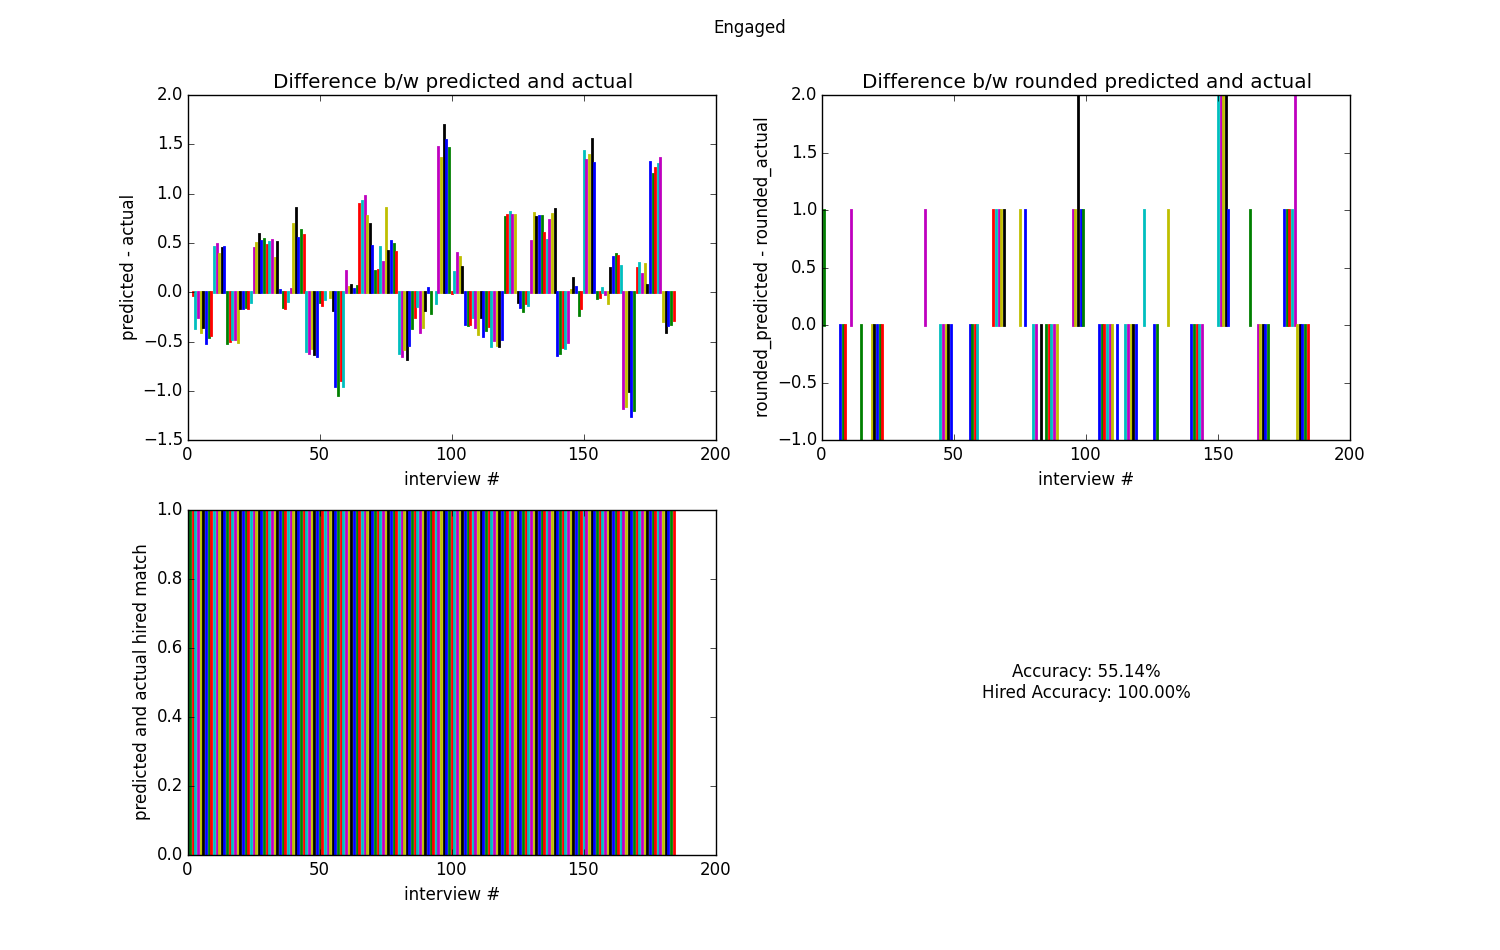
\includegraphics[width=1\columnwidth]{figures2/Engaged.png}
\end{center}
\end{figure}

\begin{figure}[H]
\begin{center}
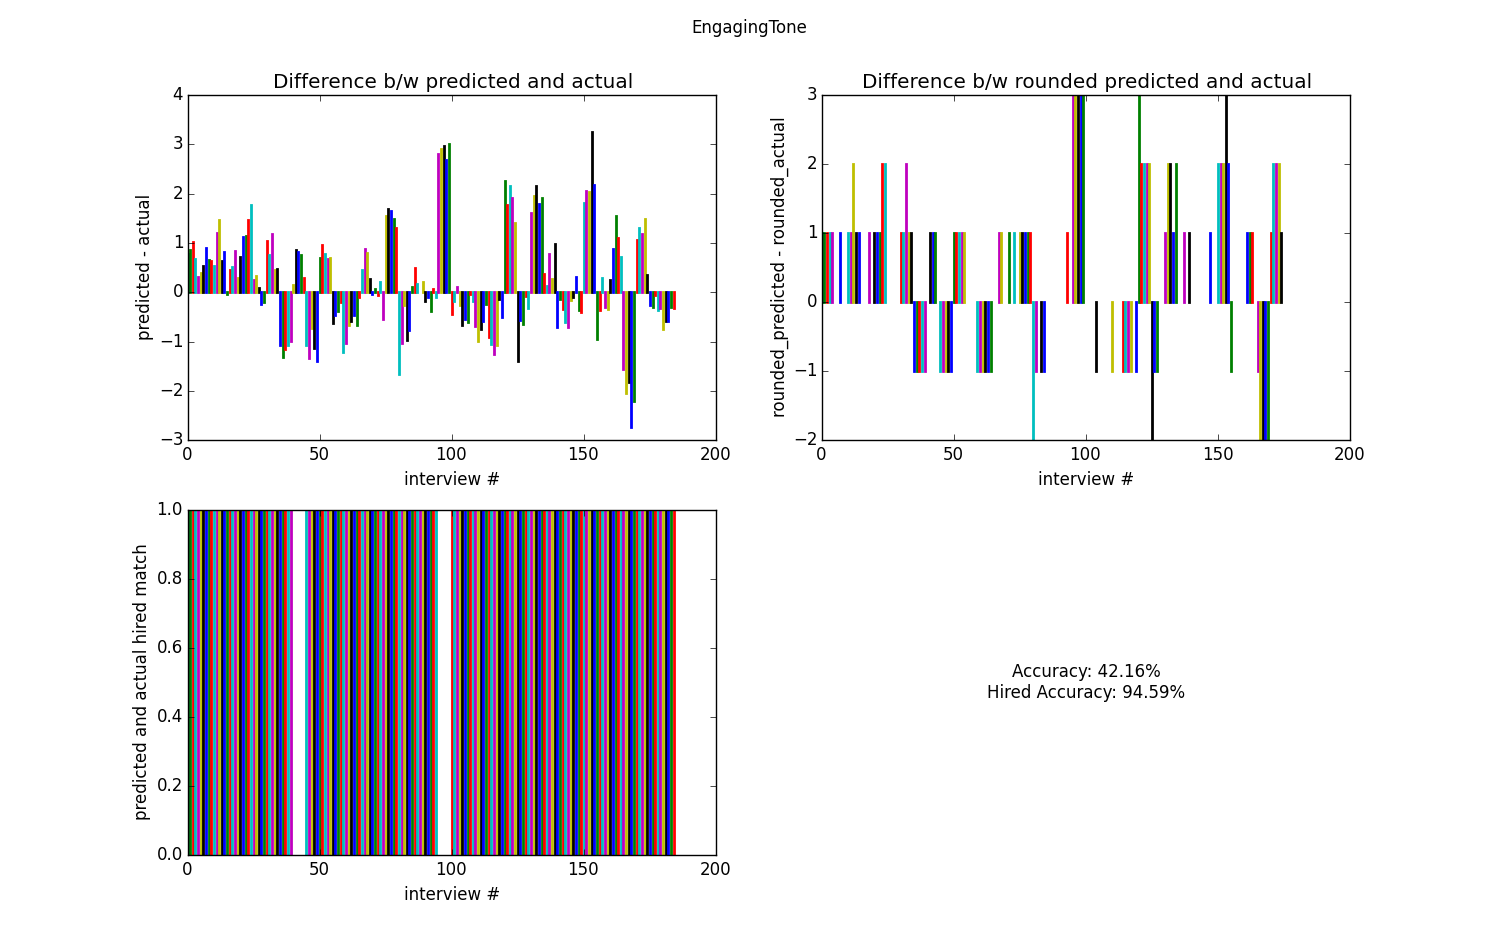
\includegraphics[width=1\columnwidth]{figures2/EngagingTone.png}
\end{center}
\end{figure}

\begin{figure}[H]
\begin{center}
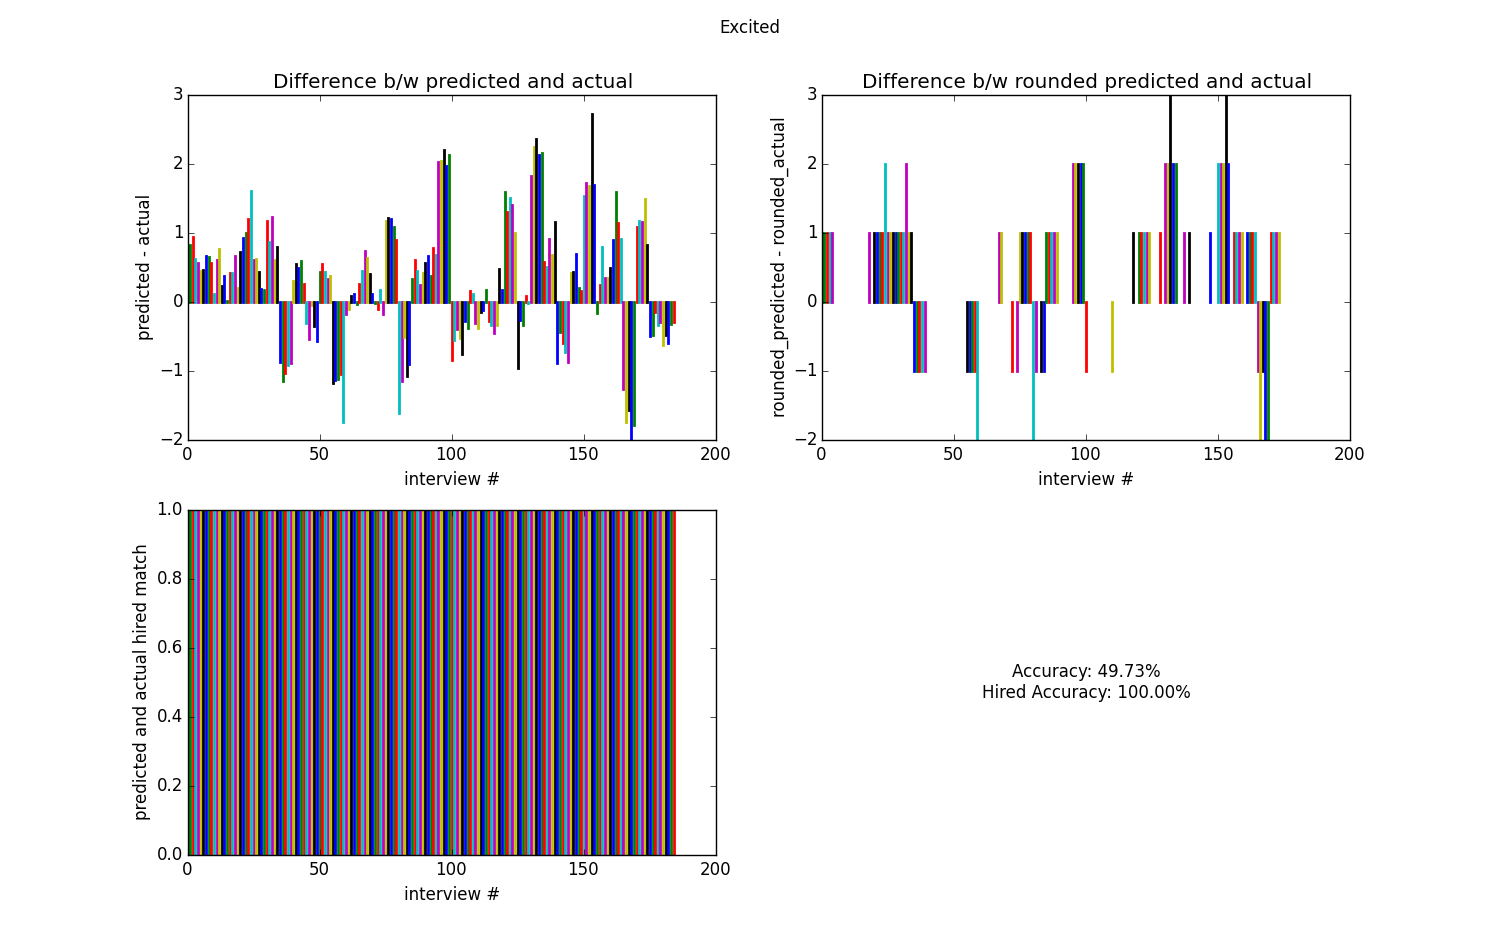
\includegraphics[width=1\columnwidth]{figures2/Excited.png}
\end{center}
\end{figure}

\begin{figure}[H]
\begin{center}
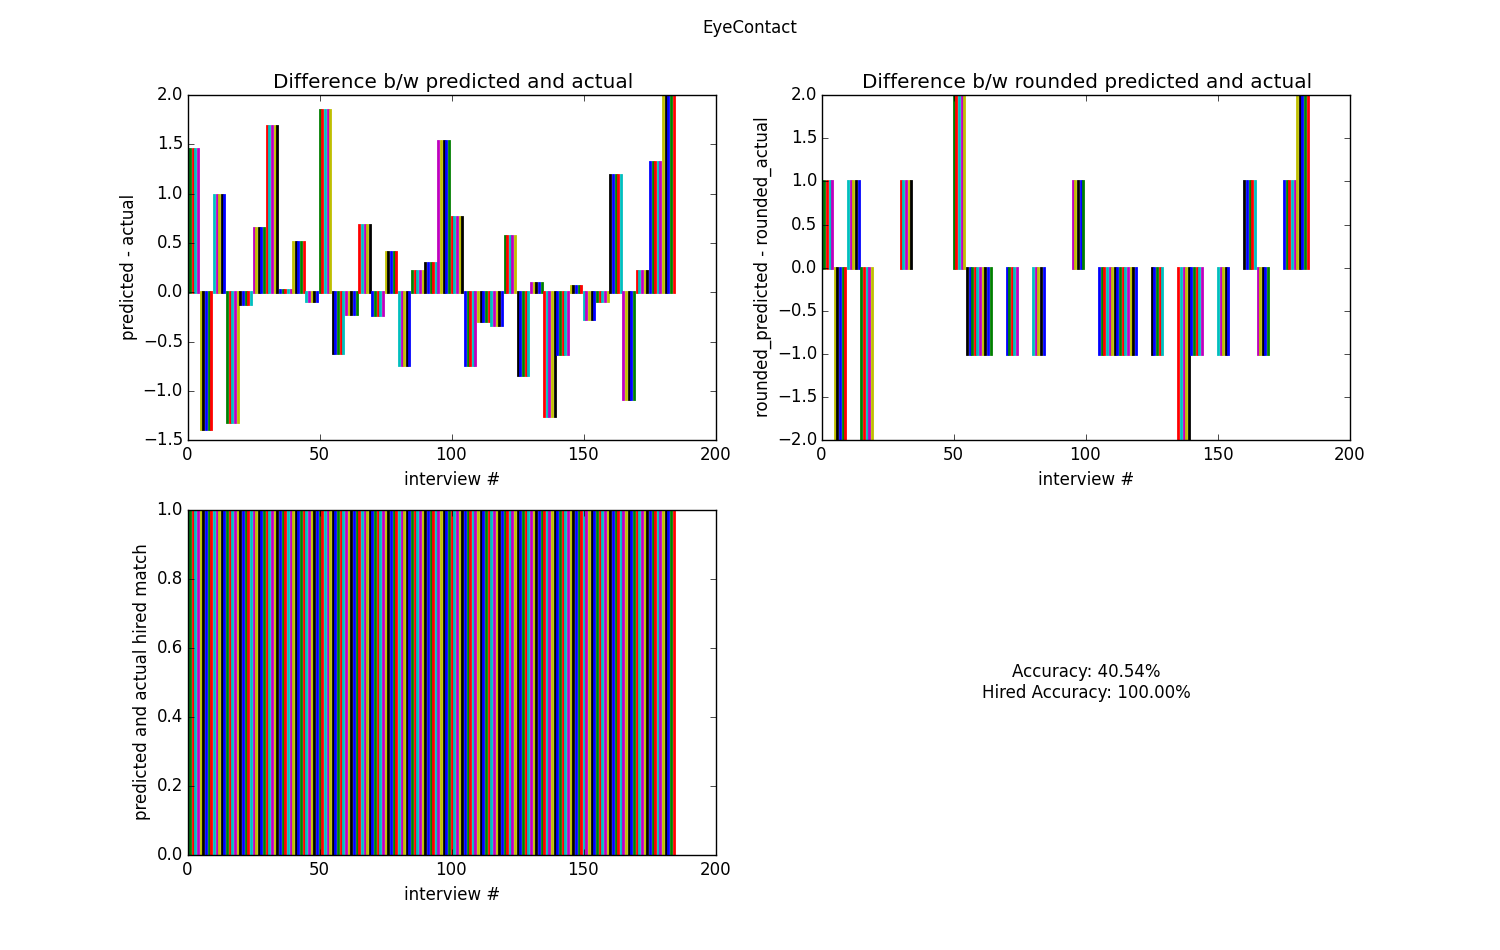
\includegraphics[width=1\columnwidth]{figures2/EyeContact.png}
\end{center}
\end{figure}

\begin{figure}[H]
\begin{center}
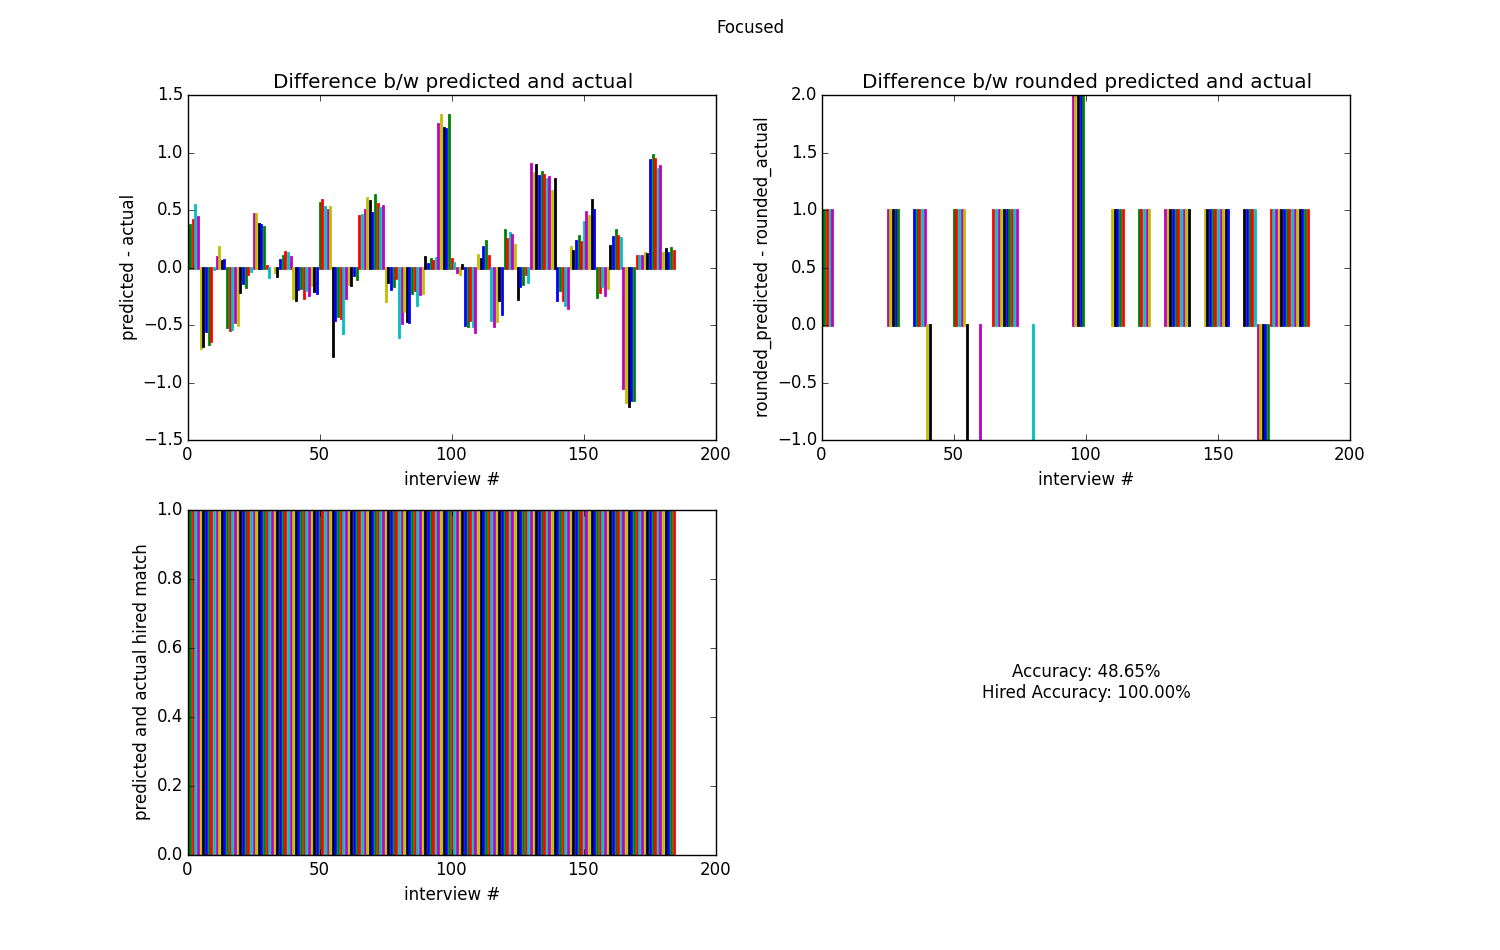
\includegraphics[width=1\columnwidth]{figures2/Focused.png}
\end{center}
\end{figure}

\begin{figure}[H]
\begin{center}
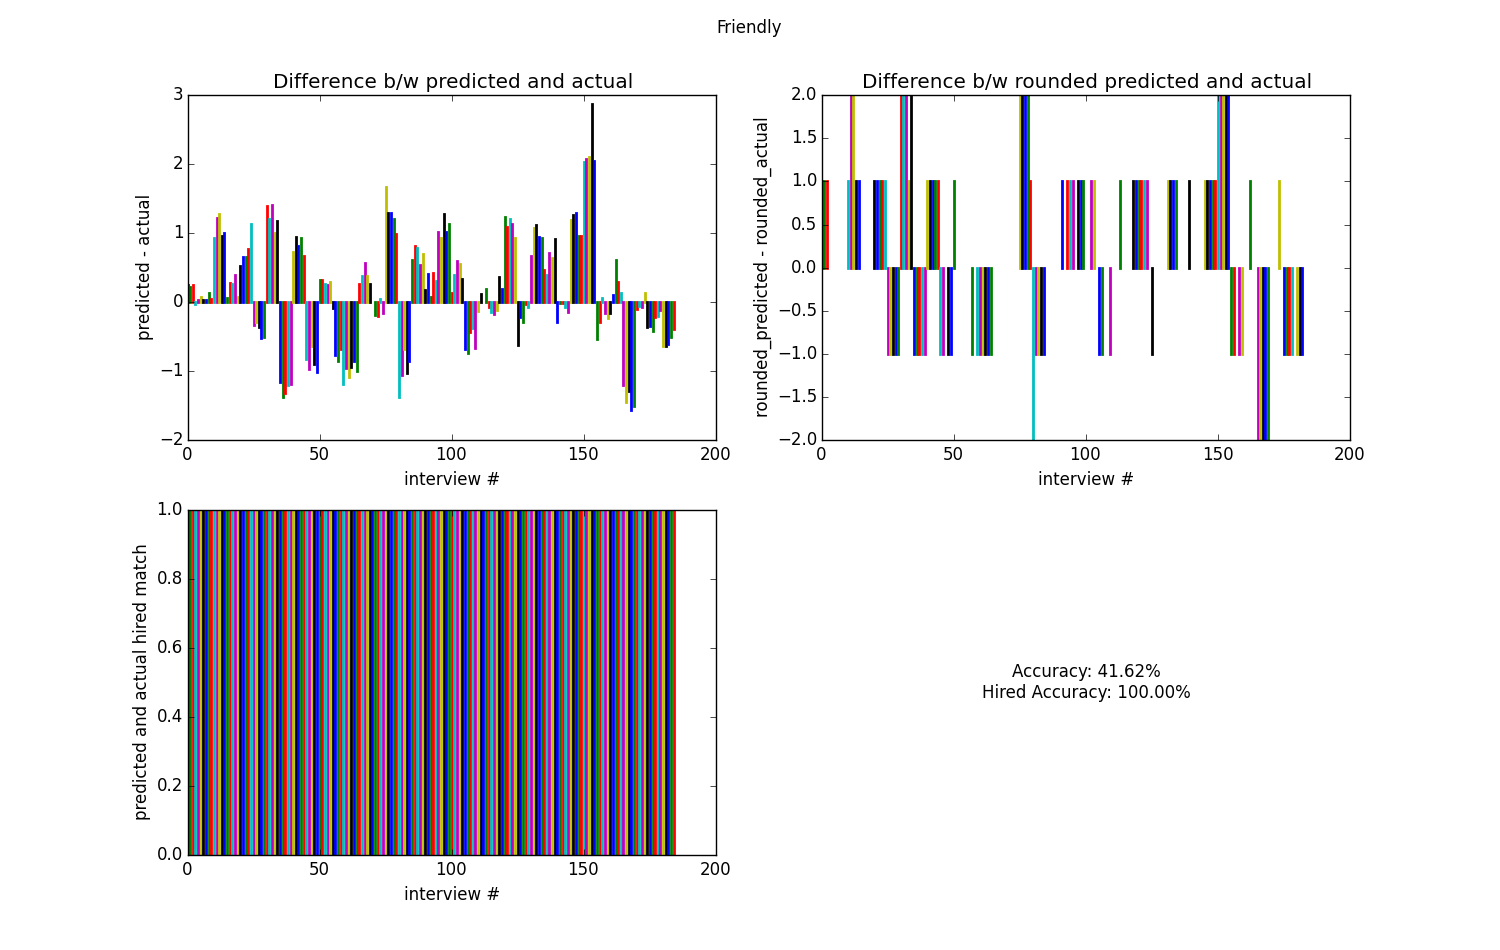
\includegraphics[width=1\columnwidth]{figures2/Friendly.png}
\end{center}
\end{figure}

\begin{figure}[H]
\begin{center}
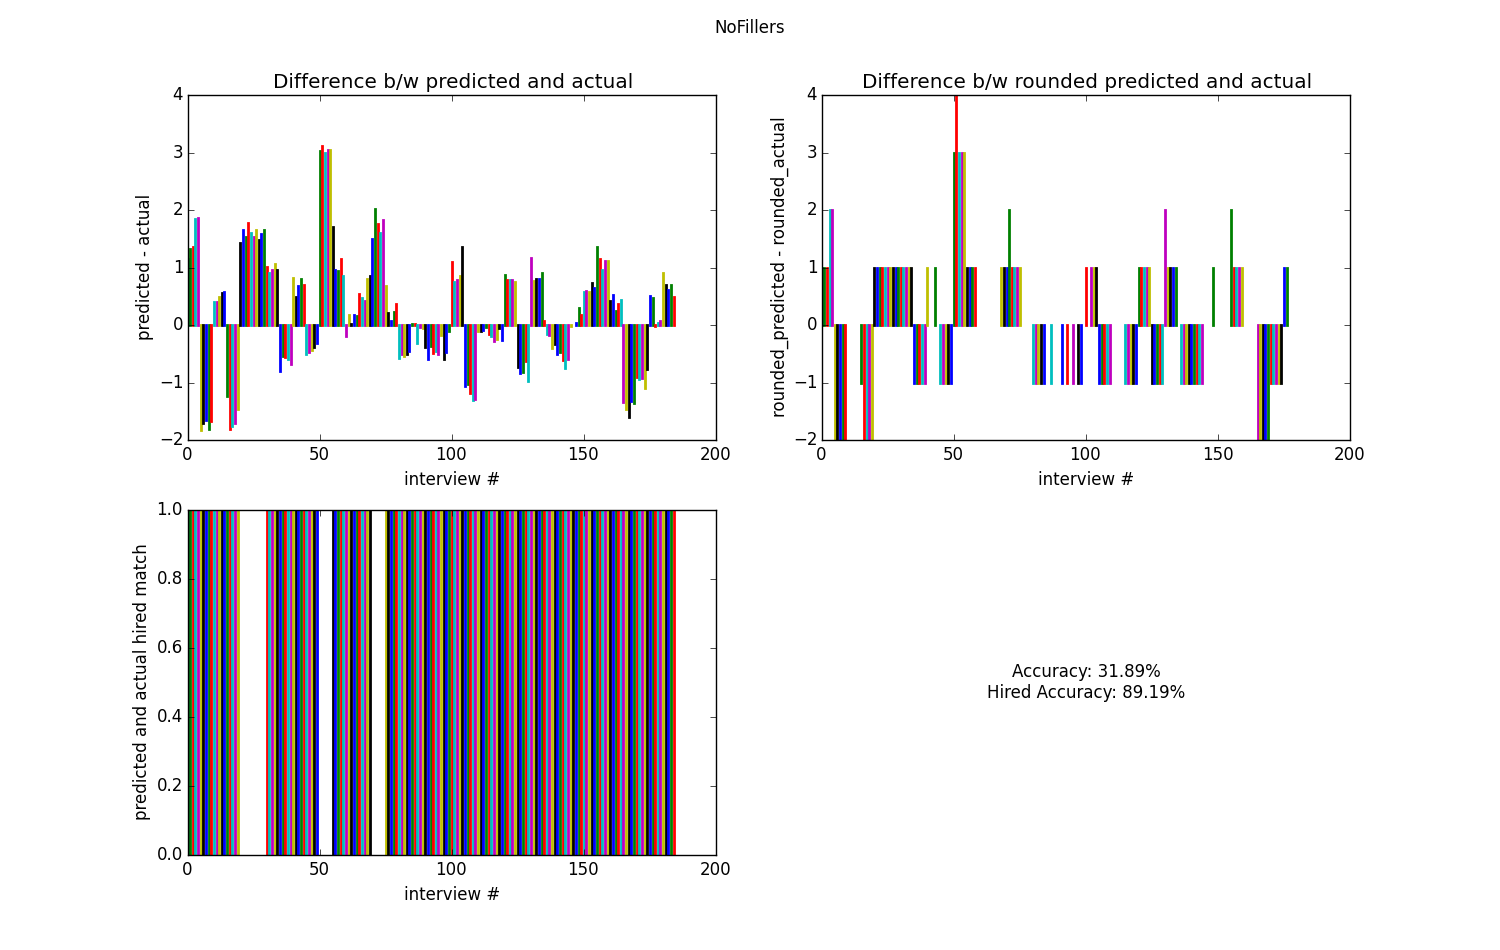
\includegraphics[width=1\columnwidth]{figures2/NoFillers.png}
\end{center}
\end{figure}

\begin{figure}[H]
\begin{center}
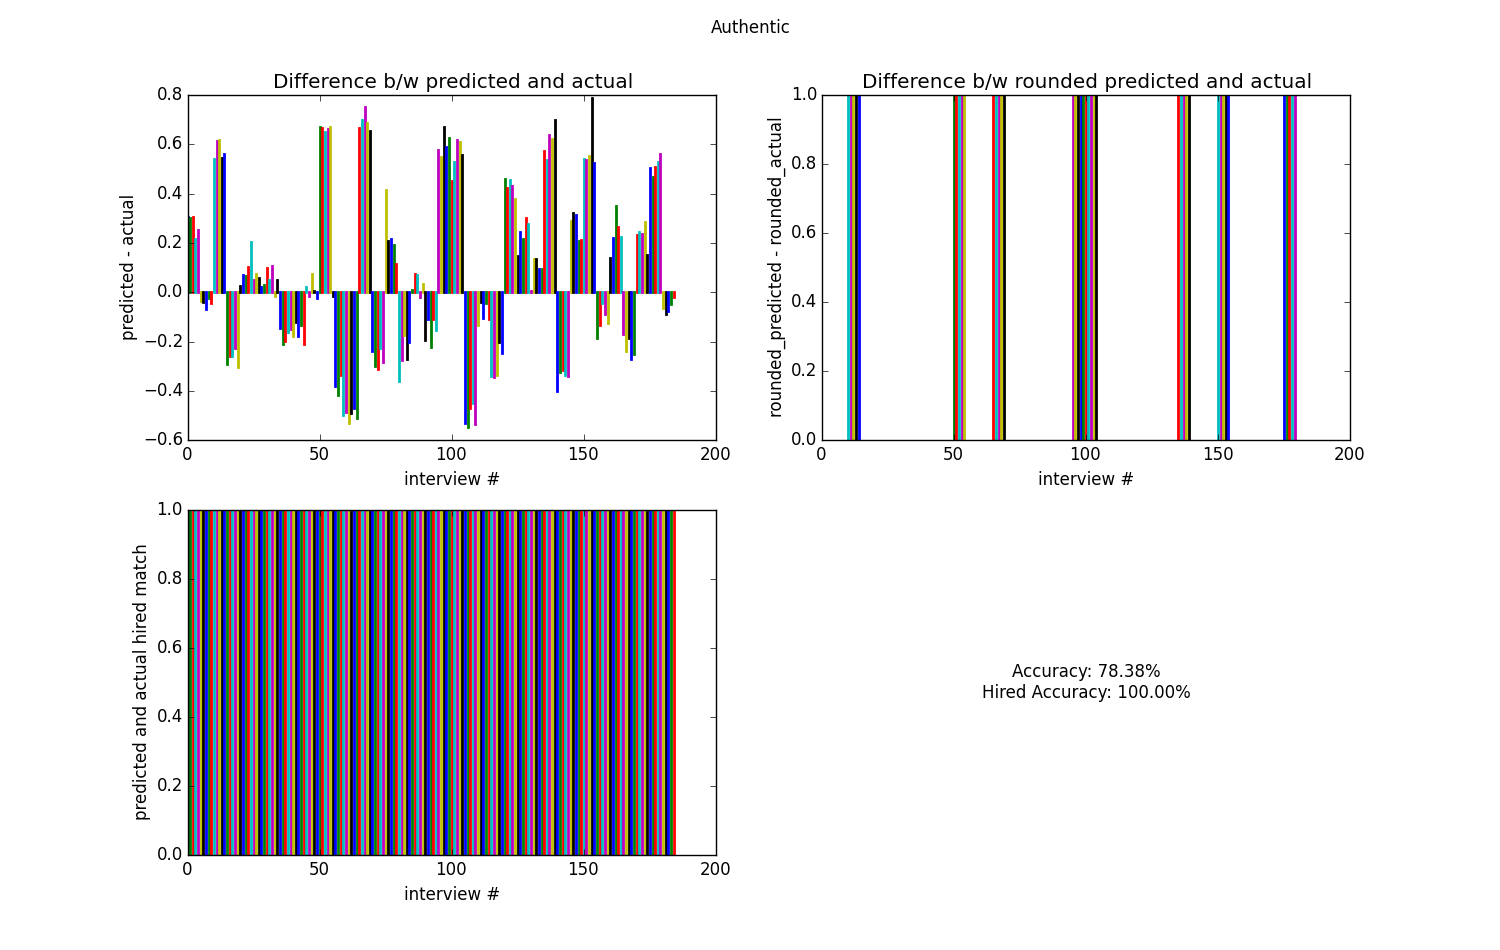
\includegraphics[width=1\columnwidth]{figures2/Authentic.png}
\end{center}
\end{figure}

\begin{figure}[H]
\begin{center}
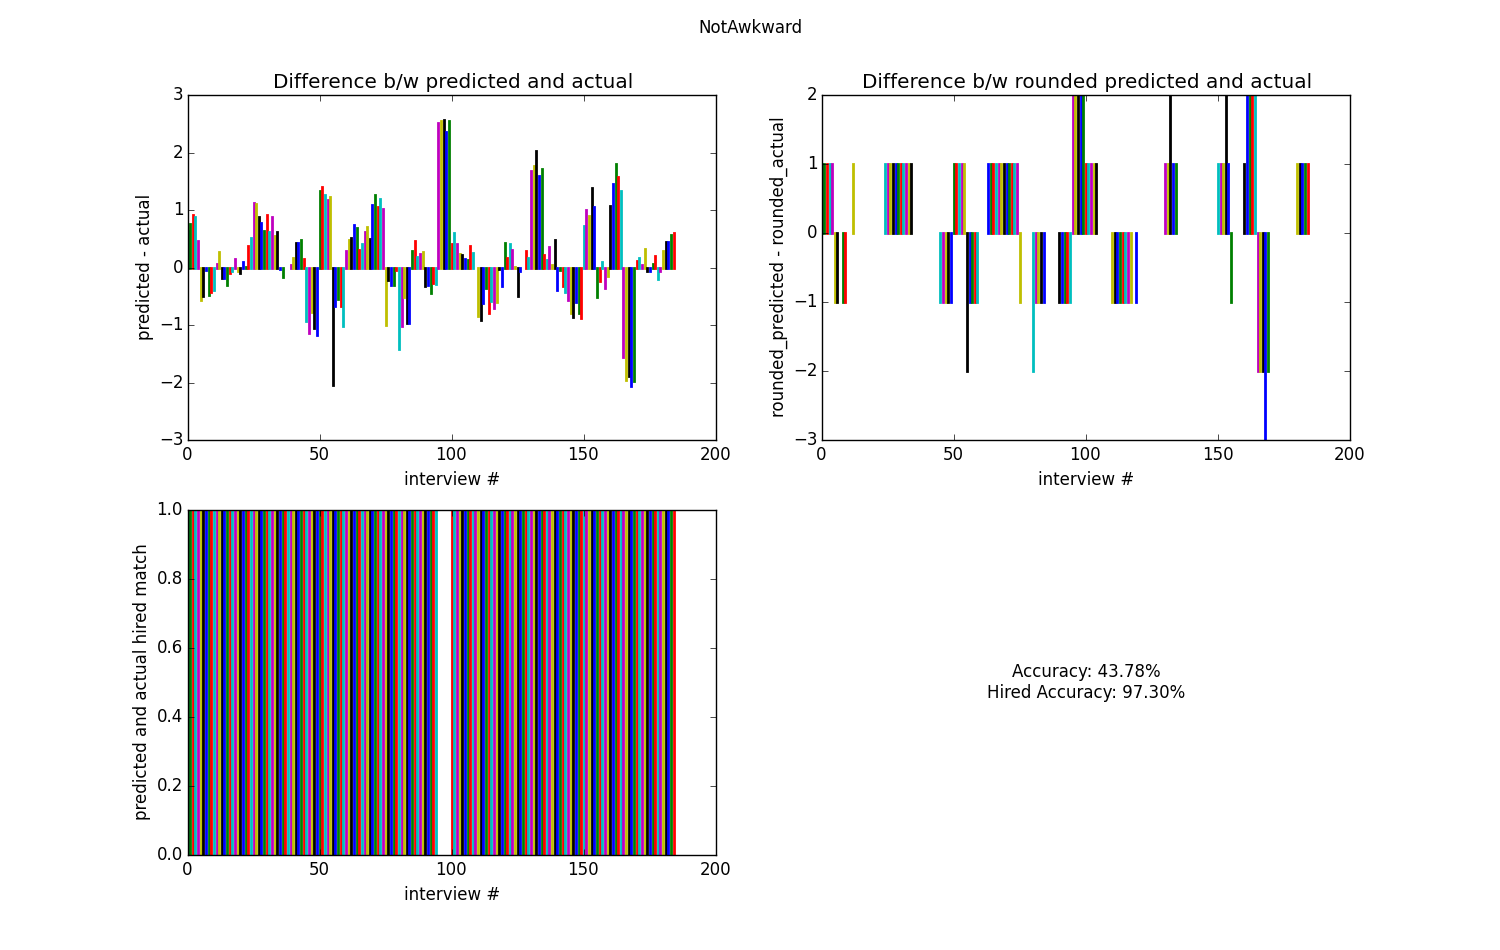
\includegraphics[width=1\columnwidth]{figures2/NotAwkward.png}
\end{center}
\end{figure}

\begin{figure}[H]
\begin{center}
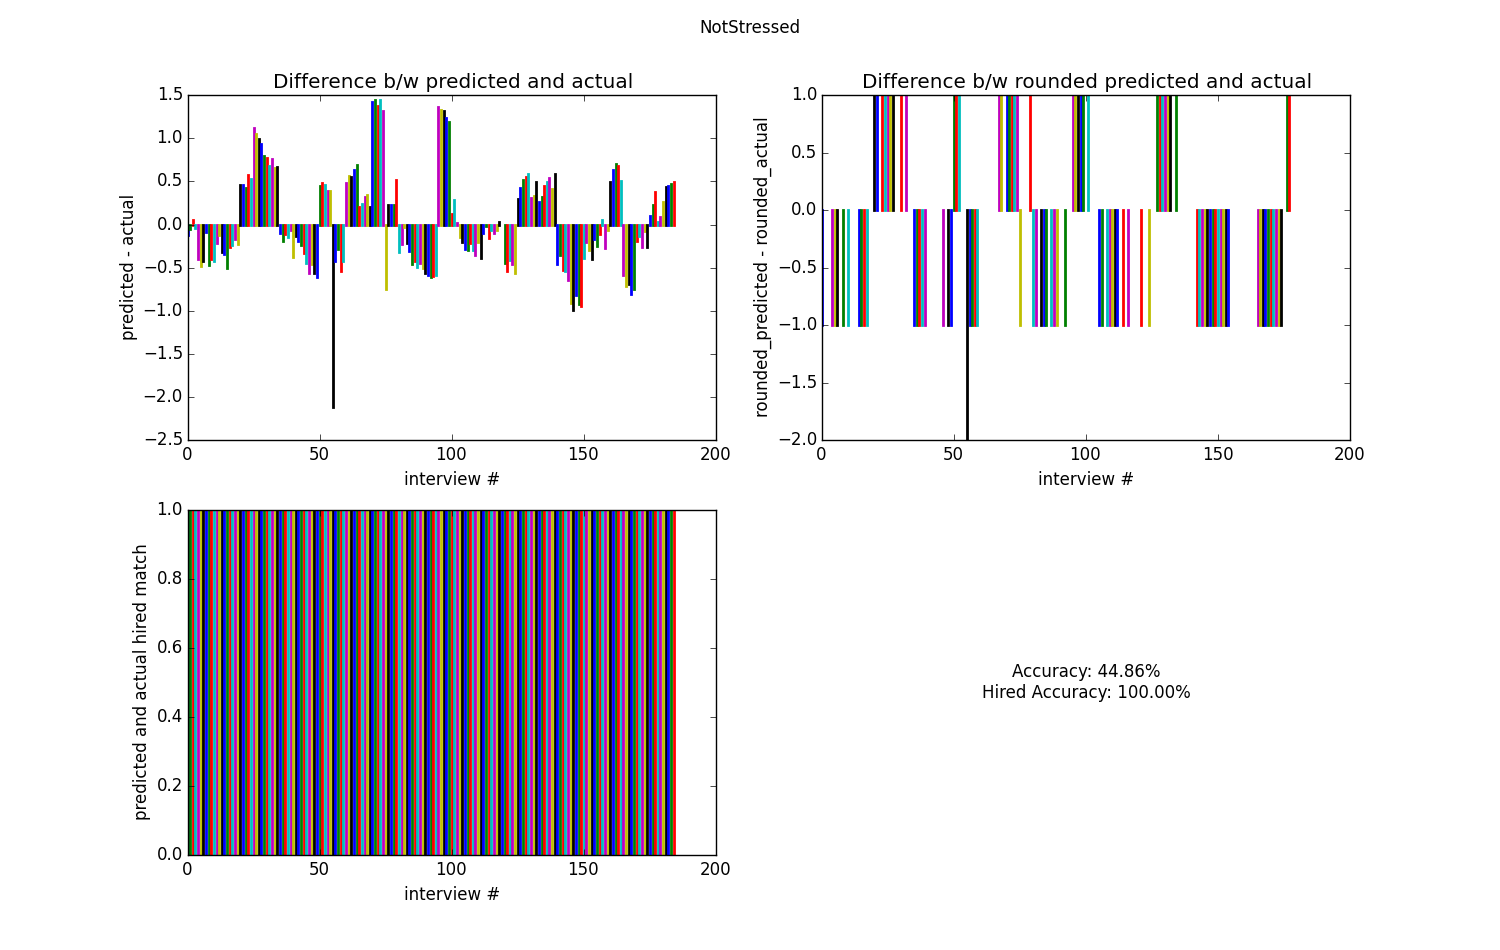
\includegraphics[width=1\columnwidth]{figures2/NotStressed.png}
\end{center}
\end{figure}

\begin{figure}[H]
\begin{center}
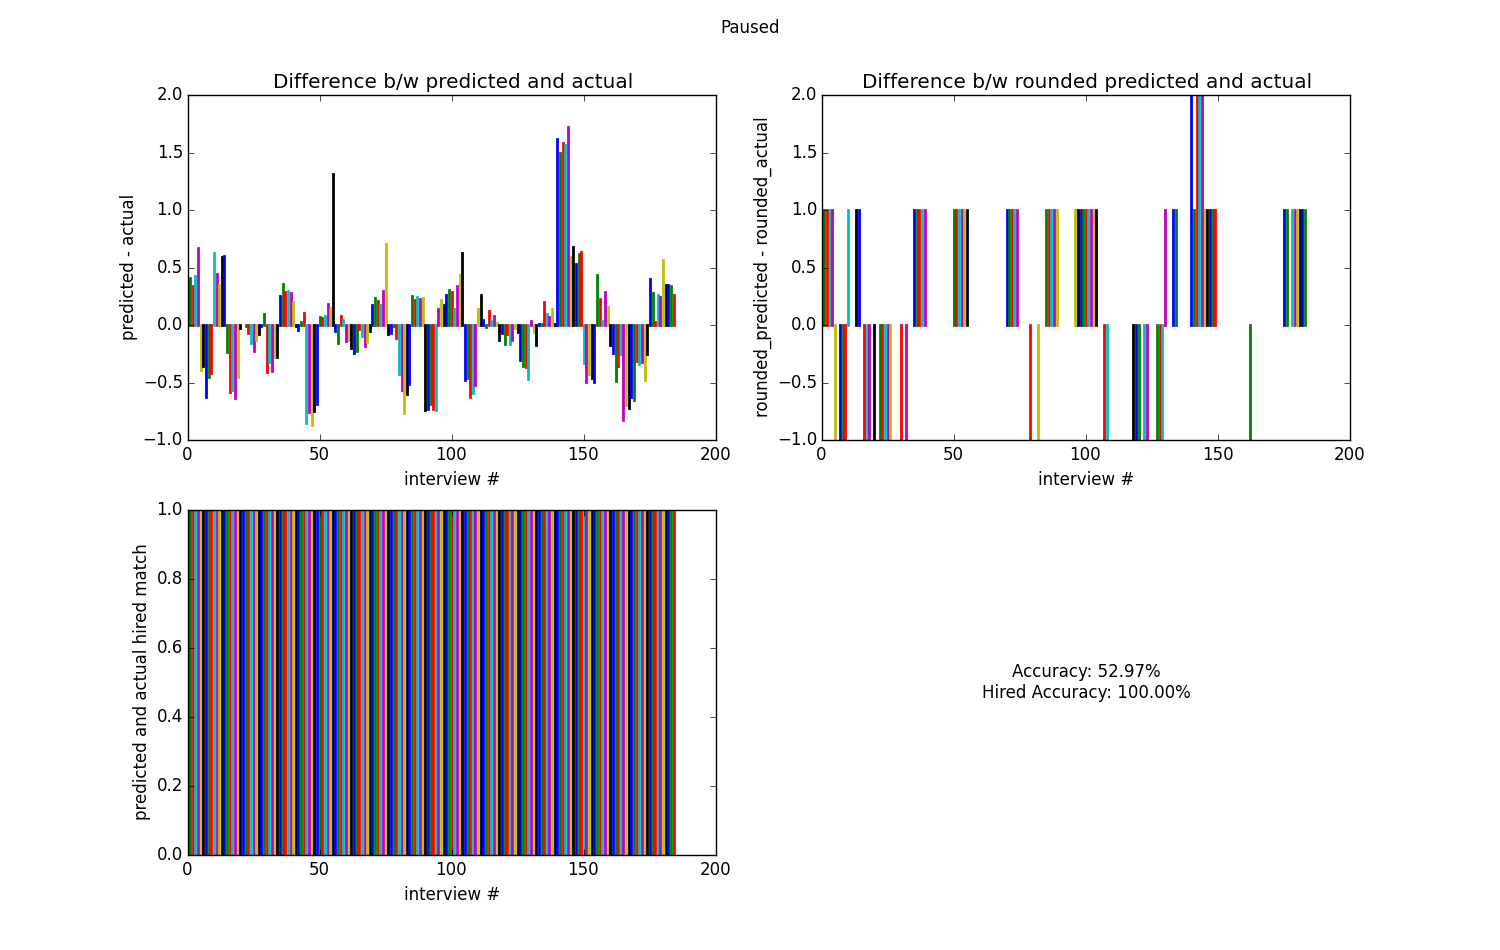
\includegraphics[width=1\columnwidth]{figures2/Paused.png}
\end{center}
\end{figure}

\begin{figure}[H]
\begin{center}
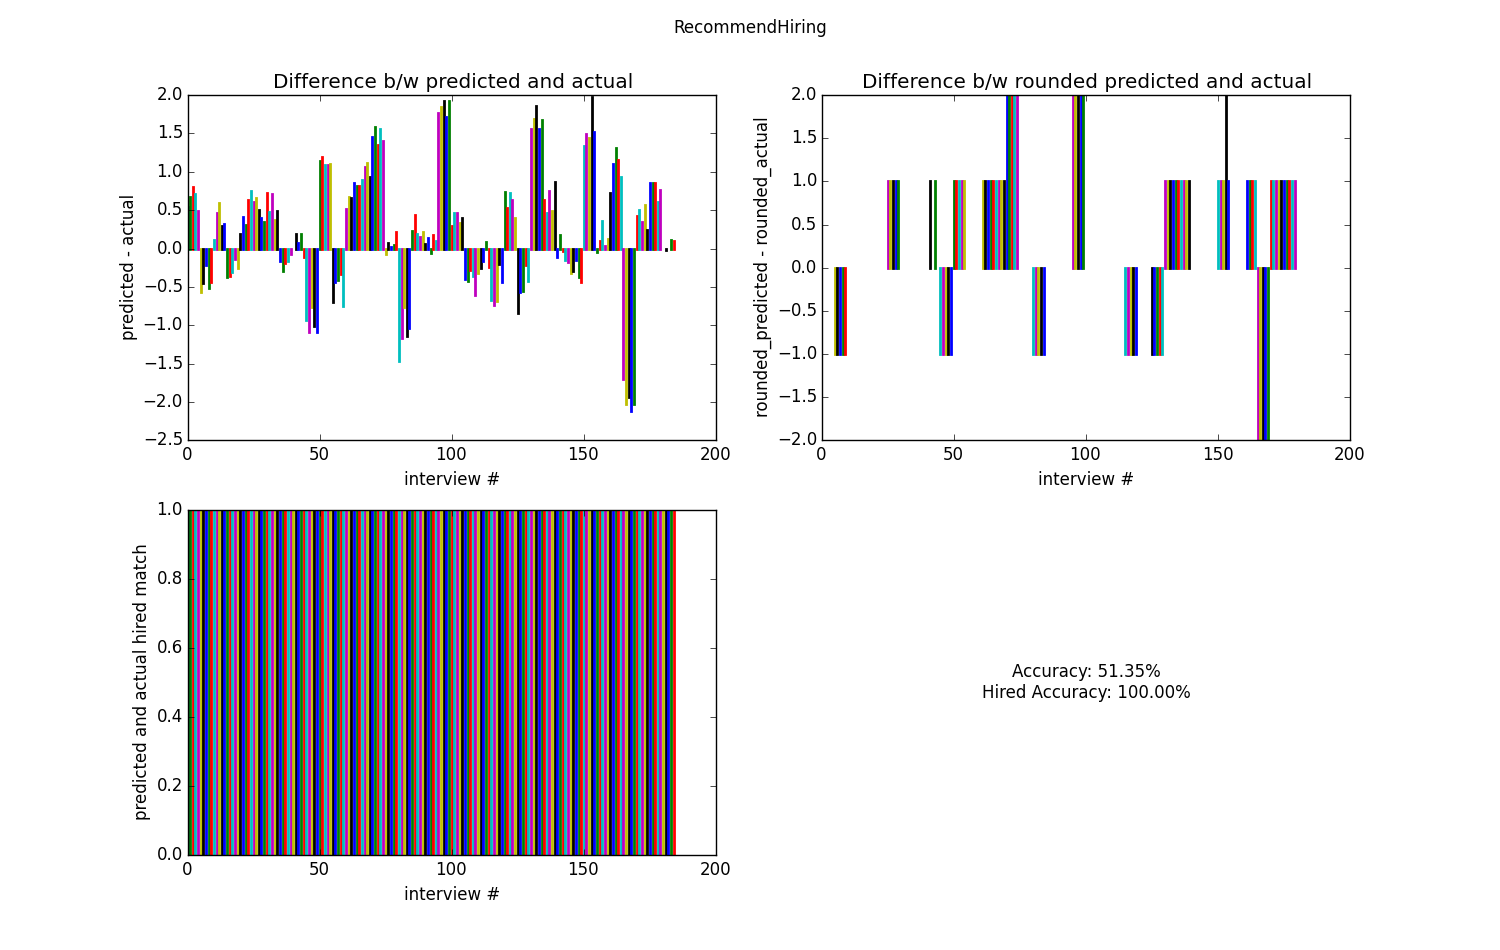
\includegraphics[width=1\columnwidth]{figures2/RecommendHiring.png}
\end{center}
\end{figure}

\begin{figure}[H]
\begin{center}
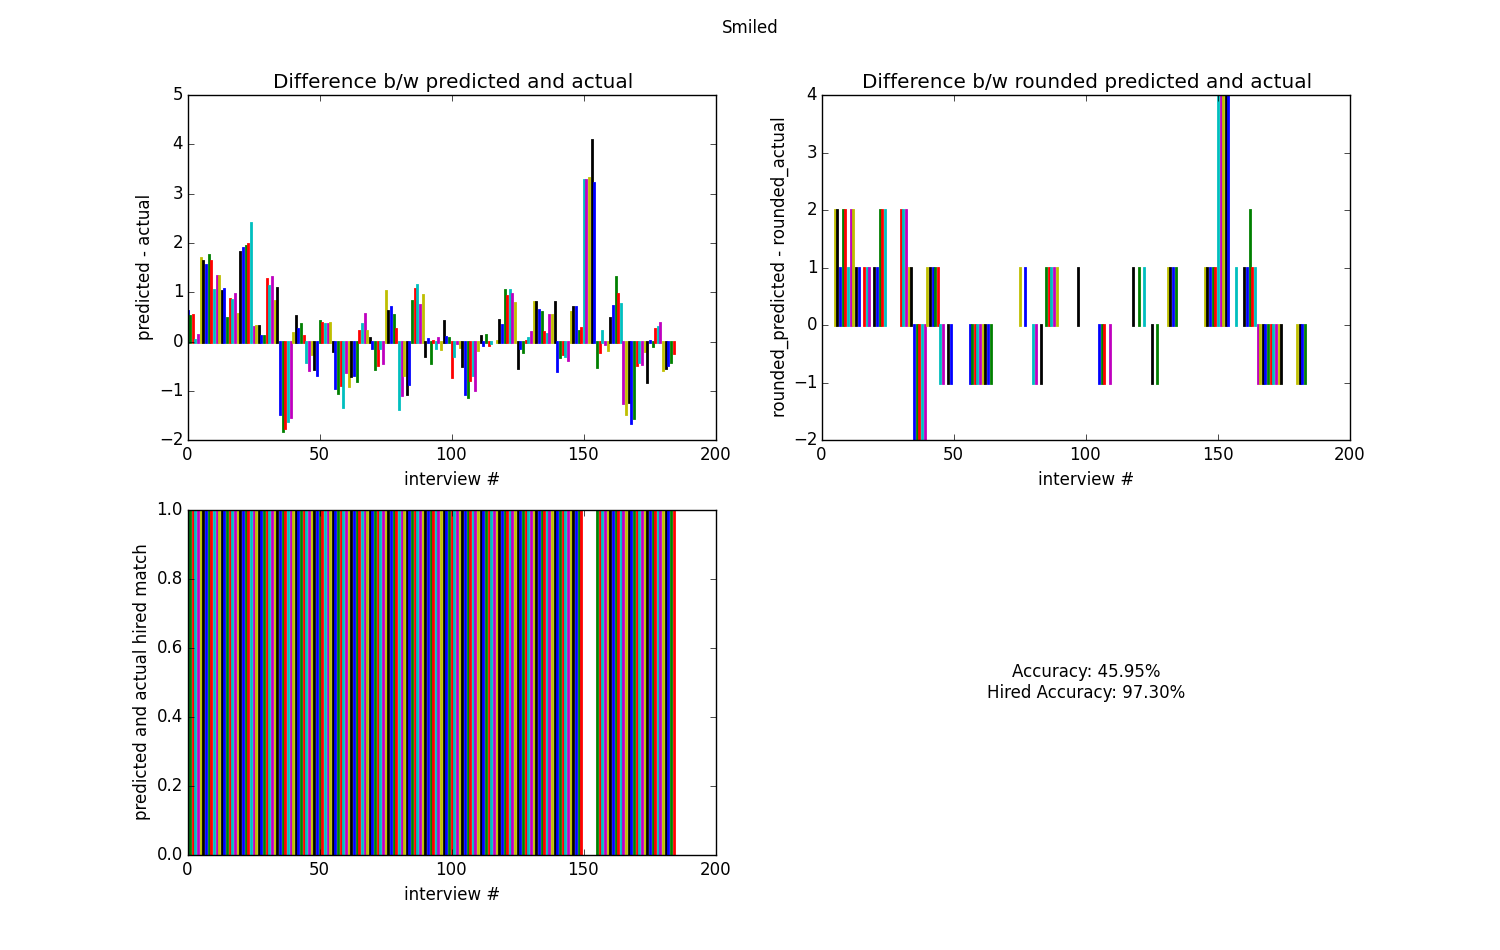
\includegraphics[width=1\columnwidth]{figures2/Smiled.png}
\end{center}
\end{figure}

\begin{figure}[H]
\begin{center}
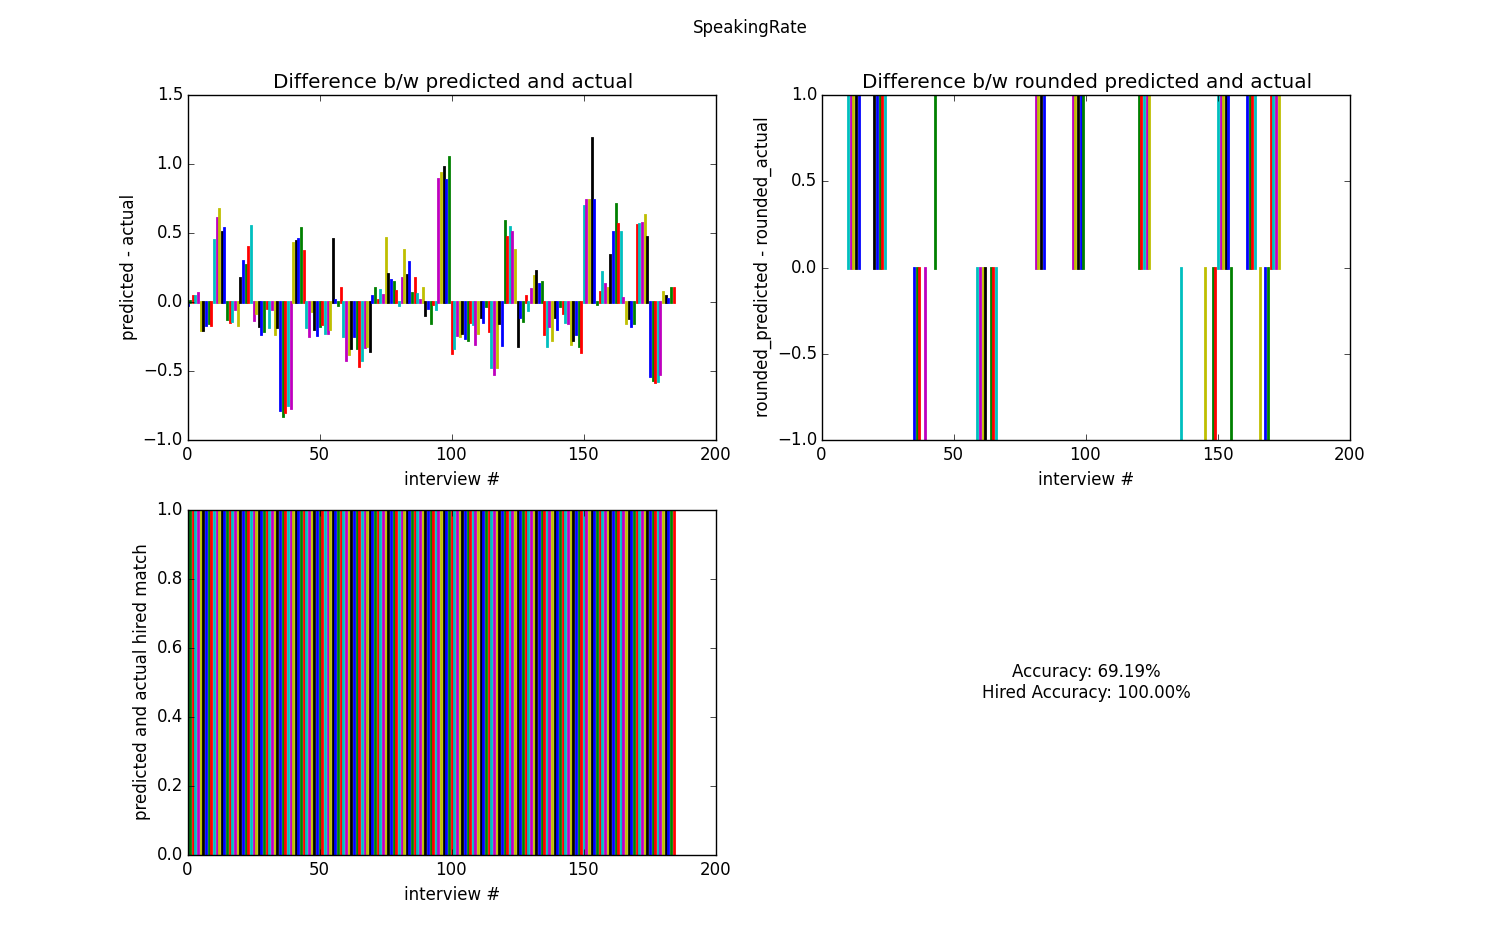
\includegraphics[width=1\columnwidth]{figures2/SpeakingRate.png}
\end{center}
\end{figure}

\begin{figure}[H]
\begin{center}
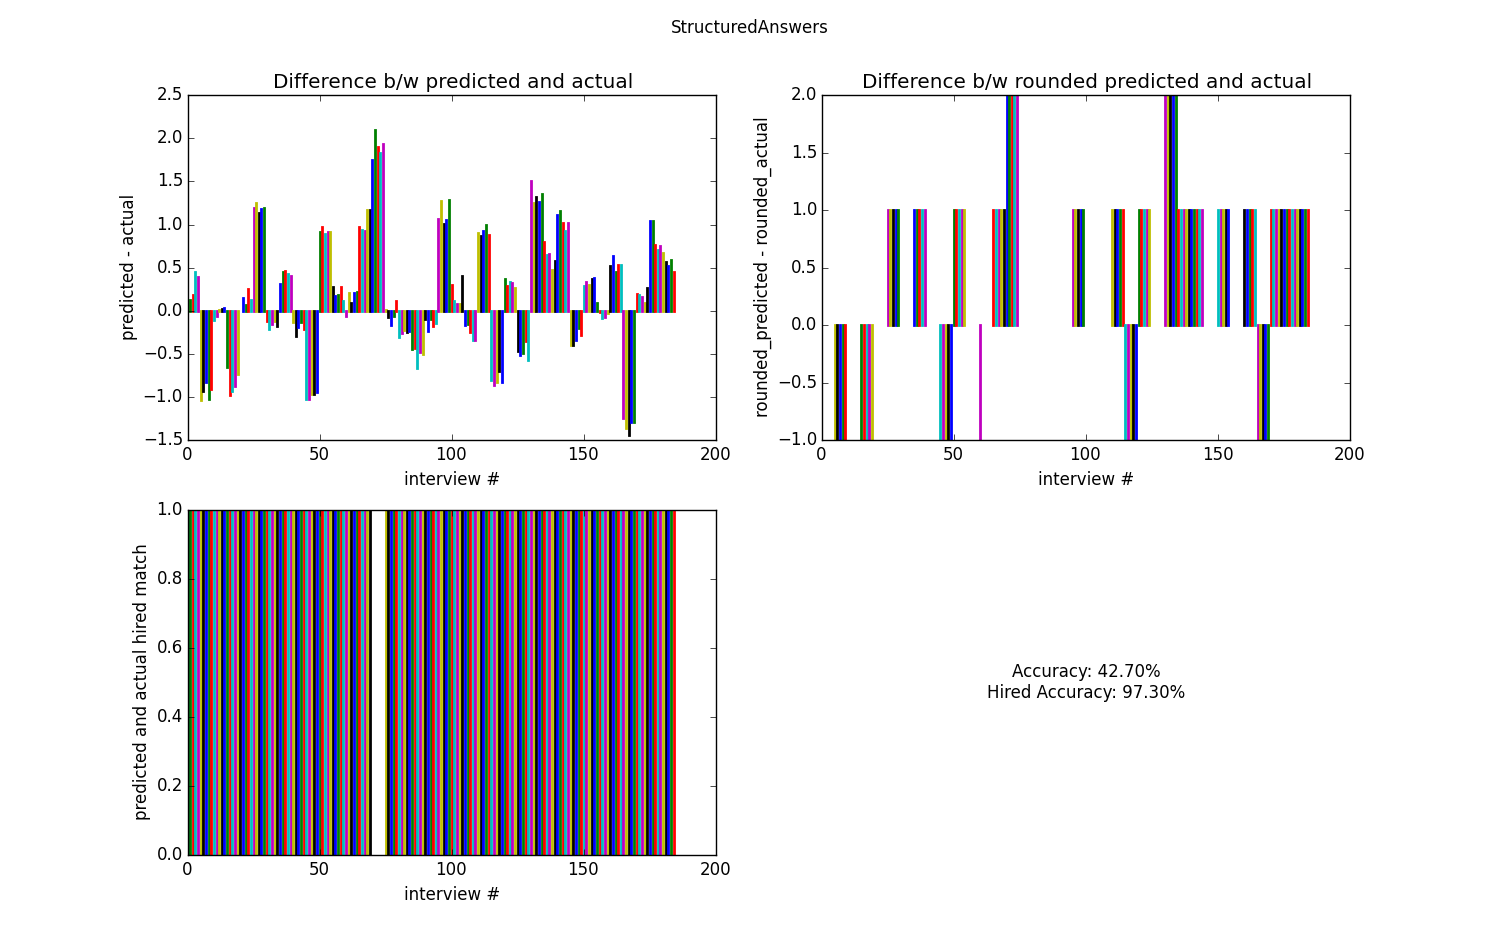
\includegraphics[width=1\columnwidth]{figures2/StructuredAnswers.png}
\end{center}
\end{figure}

From the figures above we can see that all of the assessment scores have perfect or near perfect hired accuracies. From the second graph in each of the figures we can also see that most of the scores predicted are very close and wouldn't matter much in further steps. So we consider that our regression has given good results for classification.
\subsubsection{Classification}
After using the scores of the assessment questions as features and the overall score is calculated. We find Root Mean Square Error $(RMSE)$, Root Mean Square Error over mismatches $(RMSE_{mis})$, hired accuracy with overal score limit 5/7 and overall accuracy of the result.
\begin{equation}
 RMSE = \sqrt{\frac{\sum_{i}(predicted(i)-turker(i))^2}{\textit{number of interviews}}}
\end{equation}

\begin{equation}
 RMSE_{mis} = \sqrt{\frac{\sum_{i}(predicted(i)-turker(i))^2}{count_{i}(predicted(i) \neq turker(i))}}
\end{equation}

\begin{equation}
     hired(i) = \left\{
                \begin{array}{ll}
                  1 \textit{ if predicted(i)} \geq 5 \textit{ and  turker(i)} \geq 5\\
                  1 \textit{ if predicted(i)} < 5 \textit{ and  turker(i)} < 5\\
                  0 \textit{ otherwise}\\
                \end{array}
              \right.
\end{equation}

\begin{equation}
 accuracy_{hired} = \frac{count_{i}(hired(i) == 1)}{\textit{number of interviews}}
\end{equation}

\begin{equation}
 accuracy_{overall} = \frac{count_{i}(predicted(i) == turker(i))}{\textit{number of interviews}}
\end{equation}
The following Table shows the results of the metrices discussed above. We can see that we get a good $RMSE$ value and $RMSE_{mis}$ is just slightly more than 1. The overall accuracy is 67.02\%, however this is mainly because even a difference of score 1 is considered as a mismatch. Hence, we compute hired accuracy where we say a person is hired if they get a score more than 5/7 which is 90.27\% .
\begin{center}
\begin{tabular}{ |c|c| } 
 \hline
 \textbf{Metric} & \textbf{result} \\
 \hline
 $RMSE$ &  0.588 \\ 
 \hline
 $RMSE_{mis}$ &  1.024 \\ 
 \hline
 $accuracy_{hired}$ &  90.27\% \\ 
 \hline
 $accuracy_{overall}$ &  67.02\% \\ 
 \hline
\end{tabular}
\end{center}

\section{Conclusion and Future Work}
In this project we built a computational framework using which we can analyse and measure job interviews. We used MIT Interview Dataset which consisted of 138 recordings of mock interviews of students from MIT, seeking internships. We extracted facial, prosodic and lexical features from the dataset using combinations of several techniques and tools. After measuring the inter-rater agreement using Krippendorff's Alpha we did feature analysis where we decided which set of features have to be used to measure the assessment questions. We did visual analysis of the features to find out the features which have correlation. We also used logistic regression using all the features as a feature vector to train models to predict scores of the assessment questions. By considering coeffecients of the features as a measure of relevance along with visual analysis we select features for assessment questions. Then we use SVR to predict scores of assessment questions. We use techniques such as cross-validation for each of the regressions to set the best hyper-parameters. We train a SVM classifier using the scores of assessment questions given by the turkers then use the predicted scores of assessment questions (using SVR) for testing. The classifier is trained with class variable as a whole number score between 1-7 which tells us by what extent a candidate should be hired. We use several metrices to measure the results of both SVR and SVM and find them to be good.

From the results obtained we can get a fine grain understanding of the interviews. From SVM we get overall hiring rating. From regression we get how well the interviewee has done in each of the categories. From logistic regression we know the ranking of features for regression. Using this we can give very specific details where the interviewee has or hasn’t done well.

For future work there are multiple things that we can do. First, in this approach we consider only how the interviewee performs in the interview and we don't consider the feedback provided by the interviewer. This was mainly because we can't get facial features of the interviewer as they are not visible in the videos. We can get around this by designing additional assessment questions considering just features from the interviewer. Second, we should extract more lexical features such as sentiment, domain (of the interview) dependent features, etc. Third, we can use better feature selection strategies using recurrent neural networks which require minimum manual intervention.


\section{Contribution of group members}
\begin{itemize}
 \item Suresh Alse - At first I contacted researchers from Rochester to get the MIT dataset. Then I did data cleaning and preprocessing before I extracted features using PRAAT and constructed prosodic features. Then I did visual analysis over prosodic and facial features. Then I used logistic regression to do a better feature analysis. Then using the selected features, I trained SVR models to predict scores for assessment questions. I also used cross validation to set hyper-parameters to each of the SVR models. Then I trained a SVM model from the turkers' assessment questions and predicted class of predicted assessment question scores. I used cross-validation to set the hyper-parameters. I constructed metrices to analyse SVR models. I generated graphs to visualize these metrices and calculated accuracies of the generated models. I also constructed metrices - $RMSE$, $RMSE_{mis}$, $accuracy_{hired}$ and $accuracy_{overall}$ to analyse and measure the performance of the SVM classification models. I came up with how we can use the scores to get a granular and scientific understanding of the job interviews. I also wrote a large part of this report and prepared slides for the presentation.
 
 \item Bhavishya Sharma - I helped while we were deciding the overall approach of the project. I read a lot of papers to find related work and wrote that section in this report. I did data cleaning and data transformation to make it more useful in project. I helped in coming up with validation strategies. Based on the results of visual analysis and coeffecients from logistic regression I manually selected features for some of the assessment questions. I wrote some parts of the report and final presentation.
 
 \item Jay Priyadarshi -  Wrote the code (from scratch) for calculating Krippendorff's Alpha and visualize it, which involved a lot of data preprocessing to segment the original huge annotation file. Reading through various research papers to justify why some features are more subjective and why some features are more objective which led to lower and higher values of Krippendorff’s Alpha respectively. Extracted head movements like head nods and head shakes from facial features. These were averaged and the result was used as a feature.
 
 \item Abhishek Sharma - Primary responsibility was to come up with lexical features that we could use for training our SVR model. Words like “um”, “uh”, “like” and annotations like “[long pause]” were extracted as filler words. Number of filler words per total number of words was considered as a feature. Additional features like words per second and unique words per second were also used. Used Latent Dirichlet Allocation (LDA) to learn 20 topics from interview dataset. Further extracted 20 words that were most significant to each topic (words that characterized each topic). Used the relative weights of these words in every interview as lexical features. This was done to learn what words were “important” and had an impact on the interview. Was also involved in performing feature analysis and creation of slides for the final presentation.
\end{itemize}

\bibliographystyle{apacite}
\bibliography{bibliography/converted_to_latex.bib%
}

\end{document}

